% Editorial bootstrap from the immutable source revision.
% This file is canonical and may be edited independently.

\part{All-Orders Endpoint Asymptotics}


% Source fragment: All-orders endpoint asymptotics; prefix ao.
\section{Imported inputs and the two-scale inverse problem}
\label{ao:sec:inputs}

\subsection{Forward input}

With $X=\sum_{j\ge1}2^{-j}U_j$ ($U_j$ i.i.d.\ uniform on $[0,1]$) and
$F(x)=\Probability(X\le x)$, the Laplace transform and exponent are
\begin{equation}
 M(t)=\Expectation\,\EulerE^{-tX}
 =\prod_{j\ge1}\frac{1-\EulerE^{-t/2^{j}}}{t/2^{j}},
 \qquad
 K(t)=\log M(t),
 \label{ao:eq:K-def}
\end{equation}
and the Bromwich integral
$F(x)=\frac1{2\pi\ImaginaryUnit}\int_{(\sigma)}t^{-1}\exp(xt+K(t))\Differential t$ is the
analytic source of the saddle expansion.  For small $x>0$ the exact
lower-Lambert phase is
$\lambda(x)=-\LambertW_{-1}(-Lx)/L$, i.e.\
$x=\lambda\EulerE^{-L\lambda}$ exactly, and the repository's forward
theorem states: for every fixed $N\ge1$,
\begin{equation}
 \log F(x)=
 -\frac L2\lambda^{2}+L\beta\lambda-\frac12\log\lambda
 +\Csharp+\Psi(\lambda)
 +\sum_{j=1}^{N-1}\frac{A_j(\lambda)}{\lambda^{j}}
 +\BigO_N\bigl(\lambda^{-N}\bigr),
 \label{ao:eq:forward-all-orders}
\end{equation}
uniformly in the phase.  More precisely, after the displayed terms are
subtracted the remainder is bounded in absolute value by
$C_N\lambda^{-N}$, with a constant independent of the real phase.  Every
$A_j$ is a bounded real-analytic one-periodic differential polynomial in the
Gamma--zeta fluctuation
\begin{equation}
 \Psi(u)=\sum_{k\ne0}\Psihat(k)\,\EulerE^{2\pi\ImaginaryUnit ku},
 \qquad
 \Psihat(k)=-\frac{\Gamma(-\chi_k)\,\zeta(1-\chi_k)}{L},
 \qquad
 \chi_k=\frac{2\pi\ImaginaryUnit k}{L},
 \label{ao:eq:Psi-Fourier}
\end{equation}
$\Psihat(0)=0$.  The explicit first correction and the forward
top-jet law are
\begin{equation}
 A_1(u)=\frac1{24}+\frac1{2L}
 -\frac{\Psi''(u)+\Psi'(u)^{2}}{2L^{2}},
 \qquad
 [\Psi^{(2j)}]A_j=\frac{(-1)^{j}}{2^{j}j!\,L^{2j}}.
 \label{ao:eq:A1-and-topjet}
\end{equation}
The second correction, needed for the third inverse order, is
\begin{equation}
 A_2=\frac{P_1}{24L}+\frac{2P_1+1}{4L^{2}}
 -\frac{P_1^{3}+3P_1^{2}+3P_1P_2+3P_2+P_3}{6L^{3}}
 +\frac{4P_1^{2}P_2+4P_1P_3+2P_2^{2}+P_4}{8L^{4}},
 \label{ao:eq:A2}
\end{equation}
with $P_r=\Psi^{(r)}(\theta)$, and
$A_1'=-(P_3+2P_1P_2)/(2L^{2})$.

For reference, with Euler's constant $\gamma$ and the Stieltjes convention
$\zeta(1+s)=s^{-1}+\gamma-\gamma_1s+O(s^2)$, the two constants used below are
\begin{equation}
 \Csharp=\frac{6\gamma^2+12\gamma_1-\pi^2}{12L}
 -\frac{7L}{12}-\frac12\log\pi,
 \qquad
 \CB=\frac L{12}+\frac{\pi^2-6\gamma^2-12\gamma_1}{12L}.
 \label{ao:eq:constants}
\end{equation}
In particular $\Csharp+\CB=-\tfrac12\log(2\pi)$ by direct simplification.

\subsection{Inverse prior art}

The corpus's inverse volume establishes, and this volume imports: the
leading factor and first two phase corrections
\begin{equation}
 d_1=\frac{\beta^{2}}2
 +\frac{\Csharp+\Psi(\theta)-\tfrac12\ell}{L},
 \qquad
 d_2=\frac{\Psi'(\theta)\,d_1+A_1(\theta)-\tfrac12\beta}{L};
 \label{ao:eq:d1-d2}
\end{equation}
the logarithmic corrections
$h_1=\tfrac12\ell+\kappa_0-\Psi(\theta)$ with
$\kappa_0=\beta-\tfrac L2\beta^{2}-\Csharp$, and $h_2$; the
nondegenerate first normalized cluster interval; the two-term
elasticity; and a triangular all-orders recursion.  The consolidated
results below convert that recursion into closed formulas and extend
every structural layer.

Until \cref{ao:sec:wcarrier}, the unadorned symbols $D,d_n,h_n,g_n$
always refer to this $\rho$-carrier.  The Wright--omega carrier introduced
there has a different correction and different coefficients; they will be
written $D_W,d_n^W,h_n^W,g_n^W$.  This superscript is essential: for example
$d_1=\beta^2/2+(\Csharp+\Psi-\ell/2)/L$, whereas $d_1^W=\Psi/L$.

\subsection{The two-scale problem}

For $y\downarrow0$ set
$T,\rho,z,\ell,\theta$ as in the notation table and
\begin{equation}
 \Gzero(y)=\rho\,\EulerE^{-L\rho-L\beta}
 =\frac{\sqrt T}{\EulerE\sqrt L}\,\EulerE^{-\sqrt{2LT}},
 \qquad
 \lambda(G(y))=\rho+\beta+D,
 \qquad
 D=\sum_{n\ge1}d_nz^{n}.
 \label{ao:eq:G0-D}
\end{equation}
Substituting $\lambda=\rho+\beta+D$ into
\eqref{ao:eq:forward-all-orders} and using
$-\tfrac L2\lambda^{2}+L\beta\lambda
=-T-L\rho D+\tfrac L2\beta^{2}-\tfrac L2D^{2}$ (the quadratic
collapses exactly because $T=L\rho^{2}/2$) reduces
$\log F(G(y))=-T$ to the fixed-point equation
\begin{equation}
 \boxed{\;D=z\,\Phi(z,D),\;}
 \qquad
 \Phi(z,w)=-\frac1L\mathcal R(z,w),
 \label{ao:eq:fixed-point}
\end{equation}
with the formal residual
\begin{equation}
 \mathcal R(z,w)=
 -\frac L2\beta^{2}+\frac L2w^{2}+\frac12\ell
 +\frac12\log(1+\beta z+zw)
 -\Csharp-\Psi(\theta+w)
 -\sum_{j\ge1}\frac{A_j(\theta+w)\,z^{j}}{(1+\beta z+zw)^{j}}.
 \label{ao:eq:R-def}
\end{equation}
Coefficients are computed in the two-scale ring
$\mathscr A[\ell][[z]]$, where $\mathscr A$ is the differential
algebra of one-periodic functions generated by $\Psi$ and the $A_j$:
$\ell$ and $\theta$ are treated as independent coefficient variables
and only afterwards evaluated at $\log\rho$ and $\rho+\beta$.  This
convention is forced, not cosmetic: $\theta$ winds around the circle
and $\ell$ is unbounded, so expanding either as a slow series would
destroy terms at their own order --- there is no phase-free complete
expansion (\cref{ao:sec:structure}), and the correct coefficient space
is $\RealNumbers[\ell]\otimes C^\infty(\RealNumbers/\IntegerNumbers)$.

\begin{theorem}[All-orders inverse endpoint expansion]
\label{ao:thm:all-orders}
For every fixed $N\ge1$ there are unique coefficients
$d_n,h_n,g_n\in\mathscr A[\ell]$ ($1\le n\le N$), polynomials in
$\ell$ with real-analytic one-periodic coefficients, such that as
$y\downarrow0$, uniformly in the phase,
\begin{align}
 \lambda(G(y))
 &=\rho+\beta+\sum_{n=1}^{N}\frac{d_n(\ell,\theta)}{\rho^{n}}
 +\BigO_N\Bigl(\frac{(1+\ell)^{N}}{\rho^{N+1}}\Bigr),
 \label{ao:eq:phase-expansion}\\
 \log\frac{G(y)}{\Gzero(y)}
 &=\sum_{n=1}^{N}\frac{h_n(\ell,\theta)}{\rho^{n}}
 +\BigO_N\Bigl(\frac{(1+\ell)^{N}}{\rho^{N+1}}\Bigr),
 \qquad
 \frac{G(y)}{\Gzero(y)}
 =1+\sum_{n=1}^{N}\frac{g_n(\ell,\theta)}{\rho^{n}}
 +\BigO_N\Bigl(\frac{(1+\ell)^{N+1}}{\rho^{N+1}}\Bigr).
 \label{ao:eq:G-expansion}
\end{align}
$d_n$ depends only on $\Psi,A_1,\dots,A_{n-1}$ and finitely many of
their derivatives.  By reflection, $G(1-y)=1-G(y)$ transfers every
formula to the right endpoint.
\end{theorem}

\begin{proof}
Fix $N$ and truncate the forward expansion after $A_{N-1}$.  Denote by
$\mathcal R_N$ the corresponding truncation of \eqref{ao:eq:R-def} and put
\[
 \mathcal H_N(w):=\frac Lz w+\mathcal R_N(z,w).
\]
The exact phase correction $D$ satisfies
$\mathcal H_N(D)=-E_N(D)$, where the value remainder from the forward
theorem gives $|E_N(D)|\le C_Nz^N$ uniformly in the phase.  No derivative of
$E_N$ is used below.

Substituting $D^{[N]}=\sum_{n\le N}d_nz^n$ into the formal equation and
cancelling successive powers determines $d_1,\ldots,d_N$ uniquely: at the
stage that determines $d_n$, the new coefficient occurs only in
$(L/z)D^{[N]}$ and has nonzero multiplier $L$.  Since the only explicit
$\ell$ in $\mathcal R_N$ is affine, induction gives polynomial dependence
on $\ell$; since $\Psi$ and the $A_j$ are finite differential polynomials
with normally convergent Fourier series, their Taylor coefficients are
real analytic and so are the periodic coefficients of every $d_n$.
Formal cancellation gives
\[
 |\mathcal H_N(D^{[N]})|
 \le C_N(1+\ell)^Nz^N.
\]
Both $D$ and $D^{[N]}$ are $O((1+\ell)z)$, and throughout the segment joining
them the explicitly known residual map $\mathcal H_N$ satisfies
\[
 \partial_w\mathcal H_N(w)=\frac Lz+O_N(1),
 \qquad |\partial_w\mathcal H_N(w)|\ge \frac{L}{2z}
\]
for all sufficiently small $z$.  The mean-value theorem, applied only to
$\mathcal H_N$, now yields
\[
 |D-D^{[N]}|
 \le \frac{2z}{L}
 \bigl(|E_N(D)|+|\mathcal H_N(D^{[N]})|\bigr)
 =O_N((1+\ell)^Nz^{N+1}),
\]
which is \eqref{ao:eq:phase-expansion}.  The exact Lambert identity gives
\begin{equation}
 \frac{G}{\Gzero}=(1+\beta z+zD)\,\EulerE^{-LD},
 \qquad
 H:=\log\frac{G}{\Gzero}=\log(1+\beta z+zD)-LD,
 \label{ao:eq:ratio-exact}
\end{equation}
The logarithm and exponential are analytic at the origin.  Taylor's theorem
applied to these two finite compositions therefore gives the expansion for
$H$ with remainder $O_N((1+\ell)^Nz^{N+1})$ and the expansion for
$\exp H$ with remainder $O_N((1+\ell)^{N+1}z^{N+1})$.  These are precisely
\eqref{ao:eq:G-expansion}.  Finally, reflection of the strictly increasing
CDF gives $G(1-y)=1-G(y)$ and transfers the formulas to the right endpoint.
\end{proof}

\section{The diagonal Lagrange--B\"urmann calculus}
\label{ao:sec:diagonal}

The triangular recursion computes order $n$ only after all lower
orders.  A catalytic variable turns the same fixed point into a
closed finite extraction at any single prescribed order --- the
central shared theorem of the two absorbed sources.

\begin{theorem}[Diagonal coefficient formulas]
\label{ao:thm:diagonal}
For every $n\ge1$,
\begin{equation}
 \boxed{\;
 d_n=\sum_{k=1}^{n}\frac1k\,
 [z^{\,n-k}w^{\,k-1}]\;\Phi(z,w)^{k}
 =\sum_{k=1}^{n}\frac{(-1)^{k}}{k\,L^{k}}\,
 [z^{\,n-k}w^{\,k-1}]\;\mathcal R(z,w)^{k},
 \;}
 \label{ao:eq:diagonal-dn}
\end{equation}
a finite formula: only the $z^{\,n-1}$-truncation of $\Phi$, the jets
$\Psi,\dots,\Psi^{(n-1)}$, and $A_1,\dots,A_{n-1}$ enter.  More
generally, for any formal $K(z,w)$,
\begin{equation}
 [z^{n}]\,K(z,D(z))
 =[z^{n}]\,K(z,0)
 +\sum_{k=1}^{n}\frac1k\,
 [z^{\,n-k}w^{\,k-1}]\;
 \partial_wK(z,w)\,\Phi(z,w)^{k},
 \label{ao:eq:diagonal-composition}
\end{equation}
which with $K=\log(1+\beta z+zw)-Lw$ and
$K=(1+\beta z+zw)\EulerE^{-Lw}$ gives closed diagonal formulas for
$h_n$ and $g_n$ directly.
\end{theorem}

\begin{proof}
Let $W(t,z)$ solve $W=t\,\Phi(z,W)$.  For fixed $z$, ordinary
Lagrange--B\"urmann inversion in $t$ gives
$[t^{k}]W=\tfrac1k[w^{k-1}]\Phi(z,w)^{k}$ and the composition form
$K(z,W)=K(z,0)+\sum_k\tfrac{t^{k}}k[w^{k-1}]\partial_wK\cdot\Phi^{k}$.
Since $D(z)=W(z,z)$, set $t=z$ and extract total degree $n$.
Finiteness: a term with Lagrange index $k$ asks for
$z^{\,n-k}w^{\,k-1}$, so no $A_jz^{j}$ with $j>n-k$ and at most $k-1$
phase derivatives occur.
\end{proof}

Expanding $\Phi=\sum\phi_{r,s}z^{r}w^{s}$ gives the fully unrolled
partition form
\[
 d_n=\sum_k\tfrac1k
 \sum_{r_1+\dots+r_k=n-k,\;s_1+\dots+s_k=k-1}
 \prod_j\phi_{r_j,s_j}
\]
--- convenient for proofs, while
\eqref{ao:eq:diagonal-dn} is convenient for implementation.

\begin{theorem}[Direct partial-Bell formula for $g_n$]
\label{ao:thm:direct-gn}
With $x_j=j!\,d_j$ and the partial Bell normalization
$(\sum_jd_jz^{j})^{k}
=\sum_{n\ge k}\frac{k!}{n!}\Bell_{n,k}(x_1,x_2,\dots)z^{n}$,
\begin{equation}
 \boxed{\;
 g_n=\frac1{n!}\sum_{k=1}^{n}(-L)^{k}\Bell_{n,k}
 +\frac{\beta}{(n-1)!}\sum_{k=0}^{n-1}(-L)^{k}\Bell_{n-1,k}
 +\frac1{(n-1)!}\sum_{k=1}^{n-1}k\,(-L)^{k-1}\Bell_{n-1,k},
 \;}
 \label{ao:eq:gn-direct}
\end{equation}
all $\Bell_{m,k}=\Bell_{m,k}(x_1,x_2,\dots)$; combined with
\eqref{ao:eq:diagonal-dn} this is a nonrecursive finite formula for the
arbitrary-order multiplicative coefficient.  The
logarithmic-to-multiplicative conversion is the complete-Bell
identity $g_n=\frac1{n!}\Bell_n(1!h_1,\dots,n!h_n)$, i.e.\
$ng_n=\sum_{j\le n}jh_jg_{n-j}$.
\end{theorem}

\begin{proof}
Expand the exact factorization \eqref{ao:eq:ratio-exact}: the three
lines are $[z^{n}]\EulerE^{-LD}$, $[z^{n-1}]\beta\EulerE^{-LD}$, and
$[z^{n-1}]D\EulerE^{-LD}$, each a standard partial-Bell expansion.
\end{proof}

\begin{algorithm}[Arbitrary-order symbolic generation]
\label{ao:alg:generation}
Fix an output order $N$: obtain $A_1,\dots,A_{N-1}$ (from
\eqref{ao:eq:A1-and-topjet}--\eqref{ao:eq:A2} or the saddle pipeline of
\cref{ao:sec:saddle}); Taylor-expand $\Psi(\theta+w)$, $A_j(\theta+w)$
only as far as the bidegrees require; truncate $\Phi$ at
$z^{N-1}$; evaluate \eqref{ao:eq:diagonal-dn} for each needed $n$
(no lower $d_j$ is mathematically required); and produce $g_n$ by
\eqref{ao:eq:gn-direct} or the $h$-route.  The triangular and diagonal
algorithms are complementary: the former reuses lower-order work, the
latter is an independent certificate --- the absorbed sources'
implementations verify
$d^{\mathrm{diag}}_j\equiv d^{\mathrm{tri}}_j$ symbolically for
$j\le3$ over algebraically independent jet symbols.
\end{algorithm}

\section{The explicit third correction}
\label{ao:sec:third-order}

\begin{theorem}[Closed third-order coefficients]
\label{ao:thm:third-order}
With $P_r=\Psi^{(r)}(\theta)$ and $d_1,d_2$ from
\eqref{ao:eq:d1-d2},
\begin{equation}
 \boxed{\;
 d_3=\frac1L\Bigl(
 P_1d_2+\tfrac12P_2d_1^{2}+A_1'd_1-\beta A_1+A_2
 -\tfrac L2d_1^{2}-\tfrac12d_1+\tfrac{\beta^{2}}4
 \Bigr),
 \;}
 \label{ao:eq:d3}
\end{equation}
and
\begin{equation}
 h_1=\beta-Ld_1,\quad
 h_2=d_1-\tfrac{\beta^{2}}2-Ld_2,\quad
 h_3=d_2-\beta d_1+\tfrac{\beta^{3}}3-Ld_3,
 \label{ao:eq:h123}
\end{equation}
\begin{equation}
 g_1=h_1,\qquad
 g_2=h_2+\tfrac12h_1^{2}
 =d_1-Ld_2-\beta Ld_1+\tfrac{L^{2}}2d_1^{2},
 \qquad
 g_3=h_3+h_1h_2+\tfrac16h_1^{3},
 \label{ao:eq:g123}
\end{equation}
with the direct $d$-form
$g_3=-Ld_3+(1-\beta L)d_2+L^{2}d_1d_2
+(\tfrac{\beta L^{2}}2-L)d_1^{2}-\tfrac{L^{3}}6d_1^{3}$.
\end{theorem}

\begin{proof}
Extract $[z^{2}]$ from \eqref{ao:eq:fixed-point}: the contributions are
$\tfrac L2d_1^{2}$, $\tfrac12d_1-\tfrac{\beta^{2}}4$ (from the
logarithm), $-P_1d_2-\tfrac12P_2d_1^{2}$ (Taylor transport of
$\Psi$), $-A_1'd_1+\beta A_1$ (transport of $A_1$), and $-A_2$; their
sum plus $Ld_3$ vanishes.  The $h$- and $g$-chains are the expansions
of \eqref{ao:eq:ratio-exact}.
\end{proof}

\begin{remark}[Cross-validation of the sources]
The two absorbed reports derived \eqref{ao:eq:d3} independently and
grouped it differently (one as
$-\tfrac1L\{\tfrac L2d_1^{2}+\tfrac12d_1-\tfrac{\beta^{2}}4
-P_1d_2-\tfrac{P_2}2d_1^{2}-A_1'd_1+\beta A_1-A_2\}$); the forms are
algebraically identical, and both were checked symbolically against
the triangular recursion in their independent implementations.  The
compact grouping displays the five mechanisms separately ---
quadratic saddle correction, logarithmic Jacobian, transport of
$\Psi$, transport of $A_1$, and the genuinely new $A_2$ --- and is
the stabler form for evaluation.
\end{remark}

\section{Structure laws}
\label{ao:sec:structure}

The diagonal formula does more than compute: its bidegree geometry
yields laws invisible in a triangular expansion.

\subsection{Logarithmic degrees and top logarithms}

Write $\mathcal R=\tfrac12\ell+\mathcal R_0$ with $\mathcal R_0$
independent of $\ell$, so the $z^{0}$ slice of $\Phi$ is
$\Phi(0,w)=a\ell+\phi(w)$ with
\begin{equation}
 a=-\frac1{2L},
 \qquad
 \phi(w)=\frac{\beta^{2}}2+\frac{\Csharp+\Psi(\theta+w)}L
 -\frac{w^{2}}2.
 \label{ao:eq:a-phi}
\end{equation}

\begin{theorem}[Degree and top-log laws]
\label{ao:thm:top-log}
$\deg_\ell d_1=1$ and $\deg_\ell d_n\le n-1$ for $n\ge2$, with
\begin{equation}
 [\ell^{\,n-1}]\,d_n=a^{\,n-1}\,[w^{\,n-1}]\,\phi(w)
 \qquad(n\ge2);
 \label{ao:eq:d-top-log}
\end{equation}
explicitly $[\ell]d_2=-\Psi'(\theta)/(2L^{2})$,
$[\ell^{2}]d_3=(\Psi''(\theta)-L)/(8L^{3})$, and
\[
 [\ell^{\,n-1}]d_n
 =(-1)^{n-1}\,
 \frac{\Psi^{(n-1)}(\theta)}{2^{\,n-1}L^{n}\,(n-1)!}
 \qquad(n\ge4).
\]
For the logarithmic coefficients,
$\deg_\ell h_1=\deg_\ell h_2=1$, $\deg_\ell h_n\le n-1$
($n\ge3$), with $[\ell]h_1=\tfrac12$,
$[\ell]h_2=(\Psi'(\theta)-1)/(2L)$,
$[\ell^{2}]h_3=(L-\Psi''(\theta))/(8L^{2})$, and
$[\ell^{\,n-1}]h_n
=(-1)^{n}\Psi^{(n-1)}(\theta)/(2^{n-1}L^{n-1}(n-1)!)$ for
$n\ge4$.  Finally $\deg_\ell g_n\le n$ and the multiplicative top
logarithm is \emph{universal}:
\begin{equation}
 \boxed{\;[\ell^{\,n}]\,g_n=\frac1{2^{n}n!},\;}
 \qquad
 g_n=\frac{\ell^{\,n}}{2^{n}n!}
 +\BigO_n\bigl((1+\AbsoluteValue\ell)^{n-1}\bigr)
 \text{ uniformly in }\theta.
 \label{ao:eq:universal-top-log}
\end{equation}
\end{theorem}

\begin{proof}
In \eqref{ao:eq:diagonal-dn} a product $\Phi^{k}$ has $\ell$-degree at
most $k\le n$, and for $k=n$ the coefficient requested is
$[w^{n-1}]\Phi(0,w)^{n}/n$, whose nominal $\ell^{n}$ term carries no
$w$ and dies for $n\ge2$; the $\ell^{n-1}w^{n-1}$ term takes
$a\ell$ from $n-1$ factors and $\phi$ from one, the multiplicity $n$
cancelling $1/n$ --- this is \eqref{ao:eq:d-top-log}, and expanding
$\phi$ gives the special cases.  In $H=\log(1+\beta z+zD)-LD$ the
logarithm at order $z^{n}$ involves only $d_{<n}$ (degree
$\le n-2$ for $n\ge3$), so the top logarithm of $h_n$ is
$-L[\ell^{n-1}]d_n$; orders $1,2$ are read off
\eqref{ao:eq:h123}.  For $g_n$, the only way to reach $\ell$-degree $n$
at $z$-weight $n$ in $\exp(H)$ is $(h_1z)^{n}/n!$ with the term
$\ell/2$ chosen in every factor:
$[\ell^{n}]g_n=(1/2)^{n}/n!$.  (Equivalently, in the direct
$d$-route: only $(-LD)^{n}/n!$ with $d_1=-\ell/(2L)+\BigO(1)$ from
every copy attains degree $n$, giving
$(-L)^{n}(-1/2L)^{n}/n!$ --- the two absorbed proofs of the same
law.)
\end{proof}

\begin{corollary}[First subleading multiplicative logarithm]
\label{ao:cor:subleading}
Write $h_1=\tfrac12\ell+q(\theta)$,
$q=\kappa_0-\Psi(\theta)$, and $\alpha_j(\theta)=[\ell^{\,j-1}]h_j$
($j\ge2$).  Then for $n\ge2$
\begin{equation}
 [\ell^{\,n-1}]\,g_n
 =\frac{q(\theta)}{2^{n-1}(n-1)!}
 +\sum_{j=2}^{n}\frac{\alpha_j(\theta)}{2^{n-j}(n-j)!}:
 \label{ao:eq:subleading}
\end{equation}
the first nonuniversal logarithmic layer is closed-form in the
top-log sequence of the $h_j$.
\end{corollary}

\begin{proof}
Write $H(z)=\sum_{j\ge1}h_jz^j$, so that
$1+\sum_{n\ge1}g_nz^n=\exp H(z)$.  To obtain $z^n\ell^{n-1}$, first
take $n$ copies of $h_1z$ in the exponential.  Exactly one copy must
contribute $q(\theta)$ and the other $n-1$ copies contribute $\ell/2$;
the resulting coefficient is
$q(\theta)/(2^{n-1}(n-1)!)$.

The other possibility is to take one copy of $h_jz^j$, with
$2\le j\le n$, and $n-j$ copies of $h_1z$.  The largest possible
$\ell$-degree is then $(j-1)+(n-j)=n-1$, and choosing the top term
$\alpha_j\ell^{j-1}$ from $h_j$ gives
$\alpha_j/(2^{n-j}(n-j)!)$.  Two or more factors $h_j$ with $j\ge2$
have maximal total $\ell$-degree at most $n-2$, because each such
factor loses one degree relative to its $z$-weight.  The listed cases
are therefore exhaustive, and summing them proves
\eqref{ao:eq:subleading}.
\end{proof}

The universal law explains why elementary Lambert approximations look
deceptively good --- the largest slow logarithms exponentiate as if
the periodic term were absent --- while the phase data, entering one
degree lower, are of the same size as everything else at that degree
and can never be dropped.

\subsection{Transfer of the newest periodic derivative}

\begin{theorem}[Inverse top-jet law]
\label{ao:thm:inverse-topjet}
Viewing each coefficient as a differential polynomial in $\Psi$, for
every $n\ge1$ the monomial linear in the newest jet
$\Psi^{(2n-2)}$ has
\begin{equation}
 [\Psi^{(2n-2)}]\,d_n
 =\frac{(-1)^{n-1}}{2^{n-1}(n-1)!\,L^{2n-1}},
 \qquad
 [\Psi^{(2n-2)}]\,h_n
 =[\Psi^{(2n-2)}]\,g_n
 =\frac{(-1)^{n}}{2^{n-1}(n-1)!\,L^{2n-2}}.
 \label{ao:eq:inverse-topjet}
\end{equation}
\end{theorem}

\begin{proof}
For $n\ge2$ the unique source of jet order $2n-2$ in
\eqref{ao:eq:diagonal-dn} is the $k=1$ term through
$A_{n-1}(\theta)z^{n-1}/L$: a factor $A_j(\theta+w)z^{j}$ in a term
of Lagrange index $k$ has $j\le n-k$ and gains at most $k-1$
derivatives from the $w$-extraction, so its maximal jet order
$2j+k-1\le2n-k-1$ reaches $2n-2$ only at $(k,j)=(1,n-1)$; pure
$\Psi$-factors rank lower.  The forward top-jet law
\eqref{ao:eq:A1-and-topjet} then gives the $d$-statement.  At order $n$
the logarithm in $H$ uses only $d_{<n}$ (jets $\le2n-4$), so
$h_n$ inherits $-L$ times the $d_n$ coefficient, and Bell products of
lower $h_j$ leave $g_n$ with the same newest-jet coefficient.
\end{proof}

At each order a genuinely new derivative $\Psi^{(2n-2)}$ enters
linearly with a nonzero universal coefficient: the periodic hierarchy
never closes at finite jet order, and an omission or sign error in
$A_{n-1}$ is immediately visible in $h_n,g_n$ --- a practical
computer-algebra diagnostic.

\section{Fourier-mode algebra and the analyticity strip}
\label{ao:sec:fourier}

\begin{proposition}[Finite Gamma--zeta convolutions]
\label{ao:prop:convolutions}
For a finite jet monomial
$\mathcal M=\prod_{r}\bigl(\Psi^{(r)}\bigr)^{m_r}$,
\begin{equation}
 \FourierSeriesCoefficient{\mathcal M}{k}
 =\sum_{\substack{k_{r,s}\in\IntegerNumbers\setminus\{0\}\\ \sum k_{r,s}=k}}
 \prod_{r}\prod_{s=1}^{m_r}
 (2\pi\ImaginaryUnit k_{r,s})^{r}\,\Psihat(k_{r,s}),
 \label{ao:eq:convolution}
\end{equation}
and every Fourier coefficient of every $d_n,h_n,g_n$ is a finite
linear combination of such convolutions with coefficients polynomial
in $\ell$ and belonging to the real constant algebra generated by
$L^{-1},\beta,\Csharp$ and the nonoscillatory saddle coefficients.
\end{proposition}

\begin{proof}
Termwise differentiation of \eqref{ao:eq:Psi-Fourier} gives
\[
 \Psi^{(r)}(u)=\sum_{k\ne0}(2\pi\ImaginaryUnit k)^r
 \Psihat(k)\EulerE^{2\pi\ImaginaryUnit ku}.
\]
The Gamma factor gives exponential decay in $|k|$, so this series and
all its differentiated series converge absolutely on the real axis.
The Fourier coefficient of a finite product is consequently its
ordinary Cauchy convolution.  Indexing the $m_r$ copies of
$\Psi^{(r)}$ by $s=1,\ldots,m_r$ gives exactly
\eqref{ao:eq:convolution}; absolute convergence justifies every
rearrangement.

By \cref{ao:thm:diagonal,ao:thm:direct-gn}, each fixed coefficient
$d_n,h_n,g_n$ is a finite polynomial in finitely many derivatives of
$\Psi$ and of the $A_j$.  Each $A_j$ is itself a finite differential
polynomial in $\Psi$.  Expanding these finite polynomials reduces
every nonconstant Fourier coefficient to a finite linear combination
of the displayed convolutions.  The scalar multipliers belong to the
real algebra generated by $L^{-1},\beta,\Csharp$ and the
nonoscillatory saddle constants, and their dependence on $\ell$ is
polynomial.  This is the claimed form.
\end{proof}

\begin{proposition}[Common strip]
\label{ao:prop:strip}
For every $0\le\sigma<\pi/(2L)$, all periodic coefficient functions of
all $d_n,h_n,g_n$ extend holomorphically and boundedly to
$\AbsoluteValue{\Im\theta}\le\sigma$, with normally convergent Fourier series:
Stirling on vertical lines gives
$\AbsoluteValue{\Psihat(k)}\le C_\eps\exp[-(\pi^{2}/L-\eps)\AbsoluteValue k]$, and
finite differentiation, multiplication, and coefficient extraction preserve
the exponential type.  Consequently, truncating all Fourier sums at
$\AbsoluteValue k\le K$ costs at most
$C(1+\ell)^{N}K^{\BigO(1)}
\EulerE^{-(\pi^{2}/L-2\pi\sigma)K}$ at fixed inverse order $N$ --- a few
modes suffice for high-precision real-phase evaluation, since already
$\AbsoluteValue{\Psihat(1)}=1.06271\ldots\times10^{-6}$.
\end{proposition}

\begin{proof}
Put $\tau_k=2\pi k/L$.  Stirling's estimate on vertical lines and a
polynomial vertical-line bound for $\zeta(1-\ImaginaryUnit\tau)$ give, for a
fixed exponent $A$,
\[
 |\Psihat(k)|\le C(1+|k|)^A
 \exp\!\left(-\frac{\pi^2}{L}|k|\right).
\]
Every phase derivative only inserts another power of $k$.  A finite
convolution of sequences bounded by a polynomial times
$e^{-a|k|}$ is again bounded by a (possibly larger) polynomial times
$e^{-a|k|}$: use
$|k_1|+\cdots+|k_r|\ge|k|$ and sum the remaining polynomially weighted
geometric tails.  The convolution formula of
\cref{ao:prop:convolutions} therefore yields, for every periodic
coefficient $c$ occurring through a fixed inverse order $N$,
\[
 |\FourierSeriesCoefficient{c}{k}|\le C_N(1+\ell)^N(1+|k|)^{A_N}
 e^{-\pi^2|k|/L}.
\]

On $|\Im\theta|\le\sigma$, the modulus of
$e^{2\pi\ImaginaryUnit k\theta}$ is at most $e^{2\pi\sigma|k|}$.
Since $\pi^2/L-2\pi\sigma>0$, the Weierstrass test gives normal
convergence and hence a bounded holomorphic extension to the closed
substrip.  Summing the same majorant for $|k|>K$ gives
\[
 C_N(1+\ell)^N K^{A_N'}
 e^{-(\pi^2/L-2\pi\sigma)K},
\]
after increasing the polynomial exponent to absorb the geometric
tail.  This is the stated truncation estimate.
\end{proof}

\section{Phase locking and coefficient tomography}
\label{ao:sec:tomography}

The fast phase can be frozen exactly while the endpoint is
approached, turning the formal coefficient functions into observable
limits.

\begin{theorem}[Phase-locked endpoint sequences]
\label{ao:thm:phase-locked}
Fix $u\in[0,1)$ and set
$\rho_{m,u}=m+u-\beta$,
$y_{m,u}=\exp(-\tfrac L2\rho_{m,u}^{2})$ for large integers $m$.
Then $\theta\equiv u\pmod1$ along the sequence, and
\eqref{ao:eq:G-expansion} holds with
$(\ell,\theta)=(\log\rho_{m,u},u)$, uniformly in $u$.  In
particular, the limit set of the first normalized correction
$\rho\,(G/\Gzero-1)-\tfrac12\ell$ is exactly the interval
$[\kappa_0-\max\Psi,\;\kappa_0-\min\Psi]$, every point being realized
by a phase-locked sequence.
\end{theorem}

\begin{proof}
By definition, the phase in the $\rho$-scale is
$\theta=\rho+\beta$.  Hence at $\rho=\rho_{m,u}$ it equals $m+u$ and
is congruent to $u$ modulo one.  Moreover
$\inf_{u\in[0,1]}\rho_{m,u}\to\infty$, so the uniform remainder in
\cref{ao:thm:all-orders} remains uniform after this substitution.

At first order, $g_1=h_1=\ell/2+\kappa_0-\Psi(\theta)$, and therefore
\[
 \rho\left(\frac G{\Gzero}-1\right)-\frac\ell2
 =\kappa_0-\Psi(\theta)
 +O\!\left(\frac{(1+\ell)^2}{\rho}\right).
\]
Along the phase-locked sequence the error tends to zero uniformly in
$u$, so every value of the continuous function
$u\mapsto\kappa_0-\Psi(u)$ occurs as a subsequential limit.  Conversely,
given any sequence $y_j\downarrow0$, compactness of the phase circle
provides a subsequence on which $\theta_j\bmod1\to u$; the same formula
then forces the normalized correction to converge to
$\kappa_0-\Psi(u)$.  The image of a continuous real-valued function on
the circle is the interval from its minimum to its maximum, namely
$[\kappa_0-\max\Psi,\kappa_0-\min\Psi]$.
\end{proof}

Writing $g_n(\ell,u)=\sum_{r\le n}g_{n,r}(u)\ell^{r}$, the
renormalized statistic
\begin{equation}
 \mathcal T_{N,m}(u)
 =\rho_{m,u}^{N}\Bigl\{
 \frac{G(y_{m,u})}{\Gzero(y_{m,u})}-1
 -\sum_{n<N}\frac{g_n(\log\rho_{m,u},u)}{\rho_{m,u}^{n}}
 \Bigr\}
 =g_N(\log\rho_{m,u},u)
 +\BigO_N\Bigl(\frac{(1+\log\rho_{m,u})^{N+1}}{\rho_{m,u}}\Bigr)
 \label{ao:eq:tomography}
\end{equation}
reconstructs, phase by phase, every periodic layer
$g_{N,r}(u)$ from a polynomial fit in $\log\rho$; the universal
$g_{N,N}=1/(2^{N}N!)$ supplies an exact normalization.  The endpoint
has no single asymptotic constant beyond the elementary factor: it
has a hierarchy of periodic coefficient \emph{profiles}, whose
Fourier spectra \eqref{ao:eq:convolution} are predicted explicitly.

\section{Elasticity and every inverse derivative}
\label{ao:sec:derivatives}

The value remainder in \eqref{ao:eq:forward-all-orders} cannot be
differentiated merely because it is $O(\lambda^{-N})$.  The results in this
section therefore use the following explicit derivative-stability hypothesis
on the forward saddle expansion: for every fixed $N$ and $r\ge0$, its
remainder $R_N(\lambda)$ is $C^r$ for large $\lambda$ and
\begin{equation}
 \frac{\Differential^j}{\Differential\lambda^j}R_N(\lambda)
 =O_{N,r}(\lambda^{-N})
 \qquad(0\le j\le r),
 \label{ao:eq:derivative-stable-remainder}
\end{equation}
uniformly in the real phase.  For any fixed derivative order, the usual
parameter-uniform saddle proof supplies this strengthened input by
differentiating the localized integral and repeating the same Gaussian-tail
majorant.  It is stated here because the value-only theorem used in
\cref{ao:thm:all-orders} is insufficient by itself.

Since $T=L\rho^{2}/2$ and $y=\EulerE^{-T}$, the endpoint Euler operator
acts through the two-scale derivation
\begin{equation}
 y\frac{\Differential}{\Differential y}=-\frac1{L\rho}\,\mathfrak d,
 \qquad
 \mathfrak d=\partial_\theta+z\,\partial_\ell-z^{2}\partial_z,
 \qquad
 \mathfrak d\bigl(fz^{n}\bigr)
 =(\partial_\theta f)z^{n}
 +(\partial_\ell f-nf)z^{n+1}.
 \label{ao:eq:two-scale-D}
\end{equation}

\begin{theorem}[All-orders elasticity]
\label{ao:thm:elasticity}
Assume \eqref{ao:eq:derivative-stable-remainder} to the finite order required
by the requested truncation.
The elasticity
$\mathcal E(y)=yG'(y)/G(y)$ has
$\mathcal E=\sum_{m\ge1}e_mz^{m}$ with $e_1=1$ and, for $m\ge2$
(with $h_0:=0$),
\begin{equation}
 \boxed{\;
 e_m=-\frac{\delta_{m,2}}{L}
 -\frac1L\Bigl(
 \partial_\theta h_{m-1}
 +\partial_\ell h_{m-2}-(m-2)h_{m-2}
 \Bigr);
 \;}
 \qquad
 \mathcal E
 =\frac1\rho+\frac{\Psi'(\theta)-1}{L\rho^{2}}
 +\BigO\Bigl(\frac{1+\ell}{\rho^{3}}\Bigr).
 \label{ao:eq:elasticity}
\end{equation}
\end{theorem}

\begin{proof}
Implicit differentiation of the truncated phase equation, together with
\eqref{ao:eq:derivative-stable-remainder} and the lower bound
$|\partial_w\mathcal H_N|\ge L/(2z)$ from the proof of
\cref{ao:thm:all-orders}, shows inductively that applying any fixed number of
two-scale derivatives to the omitted inverse remainder preserves its stated
symbol order.  Thus the finite expansion may be differentiated to any fixed
order covered by the hypothesis.

Apply $-(L\rho)^{-1}\mathfrak d$ to
$\log G=\ell-L\rho-L\beta+\sum h_n\rho^{-n}$: the elementary part
contributes $z-z^{2}/L$, and \eqref{ao:eq:two-scale-D} termwise gives
the recurrence; $\partial_\theta h_1=-\Psi'$ gives the two-term
form, recovering the corpus's theorem.
\end{proof}

Two complementary routes organize \emph{all} higher derivatives ---
one recursive in the derivative order, one closed via Stirling--Bell
conversion.

\begin{theorem}[Derivative hierarchy and the universal two-term law]
\label{ao:thm:derivative-hierarchy}
Assume \eqref{ao:eq:derivative-stable-remainder} through the fixed derivative
order under consideration.
The ratios $Q_m=y^{m}G^{(m)}/G$ obey the exact recurrence
$Q_{m+1}=y\tfrac{\Differential}{\Differential y}Q_m+(\mathcal E-m)Q_m$ (linear at fixed
$\mathcal E$), whose coefficient form via
\eqref{ao:eq:two-scale-D} computes every fixed $G^{(m)}$ to arbitrary
order.  Its two-term consequence is universal: for each fixed
$m\ge1$,
\begin{equation}
 \boxed{\;
 G^{(m)}(y)=(-1)^{m-1}(m-1)!\,
 \frac{G(y)}{y^{m}\rho}
 \Bigl[1+\frac{(\Psi'(\theta)-1)/L-\Hnum_{m-1}}{\rho}
 +\BigO_m\Bigl(\frac{1+\ell}{\rho^{2}}\Bigr)\Bigr],
 \;}
 \label{ao:eq:two-term-derivative}
\end{equation}
so the quantile is eventually increasing, concave, with alternating
higher derivatives near the endpoint (each fixed $m$ on its own
interval $0<y<y_m$; no uniformity in $m$ is asserted).
Alternatively, with $E=y\,\Differential/\Differential y$, $f=\log G$, and signed
Stirling numbers $s(k,j)$,
\begin{equation}
 H_k:=y^{k}f^{(k)}(y)=\sum_{j=1}^{k}s(k,j)\,E^{j}f,
 \qquad
 \frac{y^{r}G^{(r)}(y)}{G(y)}
 =\Bell_r\bigl(H_1,H_2,\dots,H_r\bigr),
 \label{ao:eq:stirling-bell}
\end{equation}
a closed finite algorithm assembling every ordinary derivative from
repeated applications of \eqref{ao:eq:two-scale-D} to $\log G$.
\end{theorem}

\begin{proof}
The recurrence is the product rule on
$G^{(m+1)}=(G^{(m)})'$.  Writing
$Q_m=a_mz(1+b_mz+\cdots)$, the operator $y\,\Differential/\Differential y$ raises the
displayed order, so $a_{m+1}=-ma_m$ and $b_{m+1}=b_m-1/m$; from
$Q_1=\mathcal E$, $a_m=(-1)^{m-1}(m-1)!$ and
$b_m=e_2-\Hnum_{m-1}$ with $e_2=(\Psi'(\theta)-1)/L$.  The
Stirling--Bell route is the classical Euler-to-ordinary conversion
followed by the complete-Bell exponential formula for
$G=\EulerE^{f}$.
\end{proof}


\section{A log-free resummation: the Wright-omega carrier}
\label{ao:sec:wcarrier}

Every coefficient of the $\rho$-scale expansion carries polynomials in
$\ell=\log\rho$.  Those logarithms are artifacts, not intrinsic
features: they enter because completing the square leaves
$\tfrac12\log\lambda$ (and the constants) outside the carrier.  The
third absorbed source resums them completely.

\subsection{The carrier}

Let $\omega$ denote the Wright omega function,
$\omega(s)+\log\omega(s)=s$ on the real line
(equivalently $\omega(s)=\LambertW_0(\EulerE^{s})$), and set
\begin{equation}
 \mathsf H:=T+\Csharp+\frac{L\beta^{2}}2,
 \qquad
 w:=\sqrt{\frac{\omega\bigl(4\mathsf H+\log(2L)\bigr)}{2L}},
 \qquad
 \vartheta:=w+\beta.
 \label{ao:eq:w-def}
\end{equation}

\begin{proposition}[Carrier equation]
\label{ao:prop:carrier-equation}
$w$ is the unique positive solution of
\begin{equation}
 T=\frac L2w^{2}-\frac{L\beta^{2}}2+\frac12\log w-\Csharp,
 \label{ao:eq:w-carrier}
\end{equation}
i.e.\ $w^{2}=\LambertW_0(2L\,\EulerE^{4\mathsf H})/(2L)$ --- the omega form
being the numerically stable one, since it never forms the
astronomically large argument.  (Newton iteration on
$\Omega+\log\Omega=S$ from the seed $\Omega_0=S-\log S+(\log S)/S$
converges immediately for large $S$.)
\end{proposition}

\begin{proof}
Multiply \eqref{ao:eq:w-carrier} by $4$ and substitute
$\Omega=2Lw^{2}$: the equation becomes
$\Omega+\log\Omega=4\mathsf H+\log(2L)$; strict monotonicity gives
uniqueness.  Note $\LambertW_0$ solves the \emph{positive}
quadratic-logarithmic equation in $T$, while $\LambertW_{-1}$
parametrizes the exact map $x\mapsto\lambda$ --- no contradiction.
\end{proof}

\begin{definition}[W-resummed carrier]
$G_W(y):=\vartheta\,\EulerE^{-L\vartheta}
=(w+\beta)\,2^{-(w+\beta)}$.
\end{definition}

Writing the exact phase as $\lambda=\vartheta+D_W$ with $z=1/w$ and
negating the forward expansion against \eqref{ao:eq:w-carrier} leaves the
residual
\begin{equation}
 0=\frac Lz D_W+\mathcal R_W(z,D_W),
 \qquad
 \mathcal R_W(z,u)=
 \frac L2u^{2}+\frac12\log(1+\beta z+zu)
 -\Psi(\vartheta+u)
 -\sum_{j\ge1}\frac{A_j(\vartheta+u)\,z^{j}}{(1+\beta z+zu)^{j}}:
 \label{ao:eq:RW}
\end{equation}
\emph{every constant and every logarithm has disappeared}.  The
entire diagonal calculus of \cref{ao:sec:diagonal} applies verbatim to
$\Phi_W=-\mathcal R_W/L$, and the ratio identity becomes
$G/G_W=\bigl(1+\tfrac{zD_W}{1+\beta z}\bigr)\EulerE^{-LD_W}$.

\begin{theorem}[Log-free all-orders expansion, with an extra order]
\label{ao:thm:W-all-orders}
With $d_m^W,h_m^W,g_m^W$ the diagonal coefficients of
\eqref{ao:eq:RW} (via \cref{ao:thm:diagonal} and its composition form),
each is a \emph{bounded real-analytic} one-periodic differential polynomial
in $\Psi,A_1,\dots,A_{m-1}$ --- after inserting the closed forward
formulas, a polynomial over $\RationalNumbers(L^{-1})$ in
$\Psi,\Psi',\dots,\Psi^{(2m-2)}$ evaluated at $\vartheta$, with no
occurrence of $\log w$ --- and, uniformly in the phase,
\begin{equation}
 \boxed{\;
 G(y)=G_W(y)\Bigl(1+\sum_{m=1}^{N}\frac{g_m^W(\vartheta)}{w^{m}}
 +\BigO_N\bigl(w^{-N-1}\bigr)\Bigr).
 \;}
 \label{ao:eq:W-expansion}
\end{equation}
Knowledge of the forward phase through $A_{N-1}$ thus determines the
inverse through order $N$ with a \emph{clean} $w^{-N-1}$ remainder
(no logarithmic grading), one power better than the forward input ---
the steep-phase Newton gain of
\cref{ao:app:proof-details} with no $(1+\ell)$ factors left to track.
\end{theorem}

\begin{proof}
Fix $N$, truncate the forward expansion after $A_{N-1}$, and let
$\mathcal R_{W,N}$ be the corresponding truncation of
\eqref{ao:eq:RW}.  The exact correction satisfies
\[
 \mathcal H_{W,N}(D_W):=\frac LzD_W+\mathcal R_{W,N}(z,D_W)
 =-E_{W,N}(D_W),
 \qquad |E_{W,N}(D_W)|\le C_Nz^N.
\]
The constant and logarithmic terms were absorbed by the carrier equation, so
all coefficients of $\mathcal R_{W,N}$ are bounded uniformly in the phase;
there is no $\ell$ variable.  The formal fixed-point equation
$D_W=z\Phi_W(z,D_W)$ therefore has unique coefficients
$D_W^{[N]}=\sum_{m\le N}d_m^Wz^m$, given by the diagonal formula of
\cref{ao:thm:diagonal}.  Each coefficient uses only finitely many Taylor
coefficients of $\Psi,A_1,\ldots,A_{m-1}$, and is consequently a bounded
real-analytic one-periodic differential polynomial with no $\log w$.

Formal cancellation gives
$|\mathcal H_{W,N}(D_W^{[N]})|\le C_Nz^N$.  Both the exact and truncated
corrections are $O(z)$, and on the segment joining them
\[
 |\partial_u\mathcal H_{W,N}(u)|
 =\left|\frac Lz+O_N(1)\right|\ge\frac{L}{2z}
\]
for small $z$.  Applying the mean-value theorem to the explicit truncated
function, not to the uncontrolled value remainder, yields
\[
 D_W-D_W^{[N]}=O_N(z^{N+1}).
\]
Finally the exact identity
\[
 \frac G{G_W}
 =\left(1+\frac{zD_W}{1+\beta z}\right)e^{-LD_W}
\]
is analytic in $(z,D_W)$ at the origin.  Substitution of the phase expansion
and Taylor's theorem give unique coefficients $h_m^W,g_m^W$ and the
$O_N(z^{N+1})$ remainder in \eqref{ao:eq:W-expansion}.  Since
$z=w^{-1}$, this is the asserted result.
\end{proof}

\subsection{First coefficients and the universal $5/24$}

With $P_r=\Psi^{(r)}(\vartheta)$ (and $P=P_0$), the diagonal
extraction gives
\begin{align}
 d_1^W&=\frac PL,
\qquad
 d_2^W=\frac{A_1-\beta/2}{L}+\frac{PP_1}{L^{2}},
\notag\\
 d_3^W&=\frac{A_2-\beta A_1+\beta^{2}/4}{L}
 +\frac{A_1P_1+A_1'P-\tfrac12(P^{2}+P+\beta P_1)}{L^{2}}
 +\frac{P(PP_2+2P_1^{2})}{2L^{3}},
 \label{ao:eq:W-d123}
\end{align}
The algebraic shape matches the $\rho$-scale recursion after its carrier term
is changed, but the coefficients are not identified: $d_m^W$ and $d_m$ belong
to different asymptotic coordinates.  The Wright--omega logarithmic
coefficients are
$h_1^W=-P$,
$h_3^W=\beta A_1-A_2-\tfrac{\beta^{2}}4
+\bigl[-A_1P_1+A_1-A_1'P
+\tfrac12(P^{2}-2\beta P+P+\beta P_1-\beta)\bigr]/L
+P(-PP_2-2P_1^{2}+2P_1)/(2L^{2})$, and, after substituting the
explicit $A_1$, every $L^{-1}$ constant in $h_2^W$ cancels:
\begin{equation}
 \boxed{\;
 h_2^W=\frac5{24}
 +\frac{P(1-P_1)}{L}
 +\frac{P_2+P_1^{2}}{2L^{2}},
 \qquad
 g_1^W=-P,
\qquad
 g_2^W=h_2^W+\frac{P^{2}}2,
 \;}
 \label{ao:eq:524}
\end{equation}
with $g_3^W=h_3^W+h_1^W h_2^W+(h_1^W)^{3}/6$.  The constant $5/24$ is a robust
invariant of the carrier normalization.  Suppressing all periodic
data while keeping the nonoscillatory parts
$A_1^{(0)}=\tfrac1{24}+\tfrac1{2L}$,
$A_2^{(0)}=\tfrac1{4L^{2}}$,
$A_3^{(0)}=-\tfrac7{2880}-\tfrac1{24L}-\tfrac1{4L^{2}}+\tfrac1{6L^{3}}$
gives the regression targets
\begin{gather}
 (h_1^W)^{(0)}=0,\quad
 (h_2^W)^{(0)}=\frac5{24},\quad
 (h_3^W)^{(0)}=-\frac{L+4}{24L},
\notag\\
 (h_4^W)^{(0)}=\frac{37L^{2}+120L+1080}{2880L^{2}},\quad
 (g_4^W)^{(0)}=\frac{199L^{2}+240L+2160}{5760L^{2}}.
 \label{ao:eq:zero-periodic}
\end{gather}

The highest-derivative law is \emph{carrier-invariant}: the W-scale
coefficients obey exactly
the right-hand coefficients in \eqref{ao:eq:inverse-topjet}, with
$(d_m,h_m,g_m)$ replaced by $(d_m^W,h_m^W,g_m^W)$ and evaluated at
$\vartheta$ (the unique source is still
$A_{m-1}$, whose top jet is normalization-independent), so the
first-harmonic contribution of this single linear top-jet monomial has
the precisely defined amplitude
\begin{equation}
 \operatorname{amp}_{\{\pm1\}}\bigl((g_m^W)_{\mathrm{top,lin}}\bigr)=
 2\AbsoluteValue{\Psihat(1)}\,
 \frac{(2\pi^{2}/L^{2})^{m-1}}{(m-1)!}
 \label{ao:eq:amplitude-law}
\end{equation}
The same identity holds for the corresponding top-jet contribution in the
$\rho$-normalization.  It describes one explicitly isolated summand, not the
amplitude or large-order growth of the complete coefficient: other
differential-polynomial terms can reinforce or cancel its first Fourier mode.

\subsection{The inversion is not the source of divergence}

\begin{theorem}[Convergent bare skeleton]
\label{ao:thm:bare-skeleton}
Set $\Psi\equiv0$, $A_j\equiv0$ in \eqref{ao:eq:RW}.  The bare reversion
$D_{\mathrm{bare}}(z)$ of
$0=\tfrac LzD+\tfrac L2D^{2}
+\tfrac12\log(1+\beta z+zD)$ is a \emph{convergent} analytic germ at
$z=0$,
\begin{equation}
 D_{\mathrm{bare}}(z)
 =-\frac{\beta}{2L}z^{2}
 +\frac{\beta^{2}}{4L}z^{3}
 +\Bigl(-\frac{\beta^{3}}{6L}+\frac{\beta}{4L^{2}}\Bigr)z^{4}
 +\BigO(z^{5}).
 \label{ao:eq:bare-series}
\end{equation}
Hence any divergence of the complete inverse series enters through
the large-order saddle data $A_j$ and the differentiated Fourier
modes --- not through formal inversion of the
quadratic--logarithmic carrier.
\end{theorem}

\begin{proof}
The equation forces $D=z^{2}V$; dividing by $z$,
$0=LV+\tfrac L2z^{3}V^{2}
+\tfrac1{2z}\log(1+\beta z+z^{3}V)$, whose logarithmic quotient is
analytic at $z=0$ with unique root $V(0)=-\beta/(2L)$ and
$V$-derivative $L\ne0$; the analytic implicit function theorem gives
the germ, and coefficient comparison the series.
\end{proof}

\begin{theorem}[Conditional Gevrey-one transfer]
\label{ao:thm:gevrey-transfer}
For $0<\sigma'<\sigma$, write
$\|f\|_\sigma=\sup_{|\Im u|\le\sigma}|f(u)|$.  Suppose $\Psi$ and every
$A_j$ extend holomorphically to $|\Im u|<\sigma$, continuously to the
closed strip, and for some $C,K\ge1$ satisfy
\[
 \|\Psi\|_\sigma\le C,
 \qquad \|A_j\|_\sigma\le CK^j j!\quad(j\ge1).
\]
Then there are constants $C',K'$, depending only on
$C,K,L,\beta,\sigma-\sigma'$, such that
\[
 \|d_m^W\|_{\sigma'}+\|h_m^W\|_{\sigma'}+
 \|g_m^W\|_{\sigma'}
 \le C'(K')^m m!\qquad(m\ge1).
\]
Thus W-resummed inversion preserves Gevrey order one; the theorem makes no
claim about a sharp exponential constant or about Borel summability.
\end{theorem}

\begin{proof}
Choose an intermediate strip
$\sigma'<\sigma_1<\sigma$ and put $\delta=\sigma-\sigma_1$.
Cauchy's estimate gives
\[
 \|\Psi^{(r)}\|_{\sigma_1}\le C\,r!\delta^{-r},
 \qquad
 \|A_j^{(r)}\|_{\sigma_1}
 \le CK^j j!\,r!\delta^{-r}.
\]
The Taylor coefficients in the auxiliary variable $u$ of
$\Psi(\vartheta+u)$ and $A_j(\vartheta+u)$ therefore lose the factor
$r!$ and are bounded by geometric powers of $\delta^{-1}$.  The expansions
of $(1+\beta z+zu)^{-j}$ and of the logarithm in
\eqref{ao:eq:RW} also have coefficients bounded by geometric powers, after
enlarging a constant depending on $L$ and $\beta$.  Consequently there are
$C_0,K_0$ such that every coefficient of total weight $r+s$ in
$\Phi_W(z,u)$ is bounded on the $\sigma_1$ strip by
\[
 C_0K_0^{r+s}(r+s)!.
\]

In the diagonal formula for $d_m^W$, a term of Lagrange index $k$ is a
product whose total weight is $m-1$.  For every decomposition
$n_1+\cdots+n_k=m-1$ one has
$n_1!\cdots n_k!\le(m-1)!$, and the number of ordered decompositions and
choices of factors is at most exponential in $m$.  Summing over
$1\le k\le m$ and absorbing these exponential counts into $K_1^m$ gives
\[
 \|d_m^W\|_{\sigma_1}\le C_1K_1^m m!.
\]
Equivalently, one may close the same majorant induction with
$\sum_{j=0}^m j!(m-j)!\le C_2m!$.

The exact logarithmic ratio and multiplicative ratio are analytic
compositions of $z$ and $D_W$ at the origin.  Their coefficient formulas are
finite convolution/Bell sums of total weight $m$; the same factorial-product
bound and exponential count give the asserted estimates for $h_m^W$ and
$g_m^W$.  Restricting from $\sigma_1$ to $\sigma'$ completes the proof.
\end{proof}

\subsection{Derivatives, numerics, and the pre-asymptotic hierarchy}

Under the derivative-stability hypothesis
\eqref{ao:eq:derivative-stable-remainder}, the W-scale remainder inherits the
same fixed-order differentiability by the implicit argument used in
\cref{ao:thm:elasticity}.  Differentiating \eqref{ao:eq:w-carrier} then gives
$\Differential T/\Differential w=Lw+(2w)^{-1}$, so with
$\mathcal H_W(w)=\sum_mh_m^W(w+\beta)w^{-m}$,
\begin{equation}
 \frac{yG'(y)}{G(y)}
 =\frac{L-(w+\beta)^{-1}-\mathcal H_W'(w)}{Lw+(2w)^{-1}}
 =\frac1w+\frac{\Psi'(\vartheta)-1}{Lw^{2}}
 +\frac{\beta+h_1^W-(h_2^W)'-\tfrac12}{Lw^{3}}
 +\BigO(w^{-4}),
 \label{ao:eq:W-elasticity}
\end{equation}
and repeated $y\,\Differential/\Differential y$ derivatives are powers of the single
operator $-\bigl(Lw+(2w)^{-1}\bigr)^{-1}\Differential/\Differential w$ --- no second
inversion, consistent with \cref{ao:sec:derivatives}.

On the exact dyadic quantiles the improvement over the
$\rho$-carrier is dramatic --- the bare W-carrier already beats the
$\rho$-scale's two-correction approximant at small $n$:

\begin{center}
\small
\begin{tabular}{@{}rrrrrr@{}}
\toprule
$n$ & $w$ & carrier only & order 1 & order 2 & order 3 \\
\midrule
5   & 6.066   & $-4.79\times10^{-3}$ & $-4.79\times10^{-3}$ & $8.58\times10^{-4}$ & $-4.13\times10^{-4}$ \\
10  & 11.845  & $-1.35\times10^{-3}$ & $-1.35\times10^{-3}$ & $1.36\times10^{-4}$ & $-3.32\times10^{-5}$ \\
20  & 22.680  & $-3.84\times10^{-4}$ & $-3.84\times10^{-4}$ & $2.11\times10^{-5}$ & $-2.95\times10^{-6}$ \\
40  & 43.566  & $-1.07\times10^{-4}$ & $-1.07\times10^{-4}$ & $3.16\times10^{-6}$ & $-2.30\times10^{-7}$ \\
80  & 84.491  & $-2.87\times10^{-5}$ & $-2.87\times10^{-5}$ & $4.50\times10^{-7}$ & $-1.66\times10^{-8}$ \\
160 & 165.444 & $-7.55\times10^{-6}$ & $-7.55\times10^{-6}$ & $6.11\times10^{-8}$ & $-1.14\times10^{-9}$ \\
\bottomrule
\end{tabular}
\captionof{table}{Relative errors of the W-resummed approximants
$G_W\exp(\sum_{j\le r}h_j^W/w^{j})$ at $y_n=F(2^{-n})$.  Compare
\cref{ao:tab:dyadic-errors}: order for order the W-scale wins throughout
(at $n=160$, third order $-1.14\times10^{-9}$ versus
$4.92\times10^{-8}$; second order $6.1\times10^{-8}$ versus
$-3.6\times10^{-6}$), and the \emph{bare} carrier alone outperforms
the $\rho$-scale's full $h_2$-approximant through
$n\approx40$ ($-1.07\times10^{-4}$ versus $-1.43\times10^{-4}$ at
$n=40$; the comparison reverses beyond $n\approx80$ as the
$\rho$-corrections catch up) by absorbing the logarithmic drift.}
\label{ao:tab:W-errors}
\end{center}

\begin{figure}[htbp]
\centering
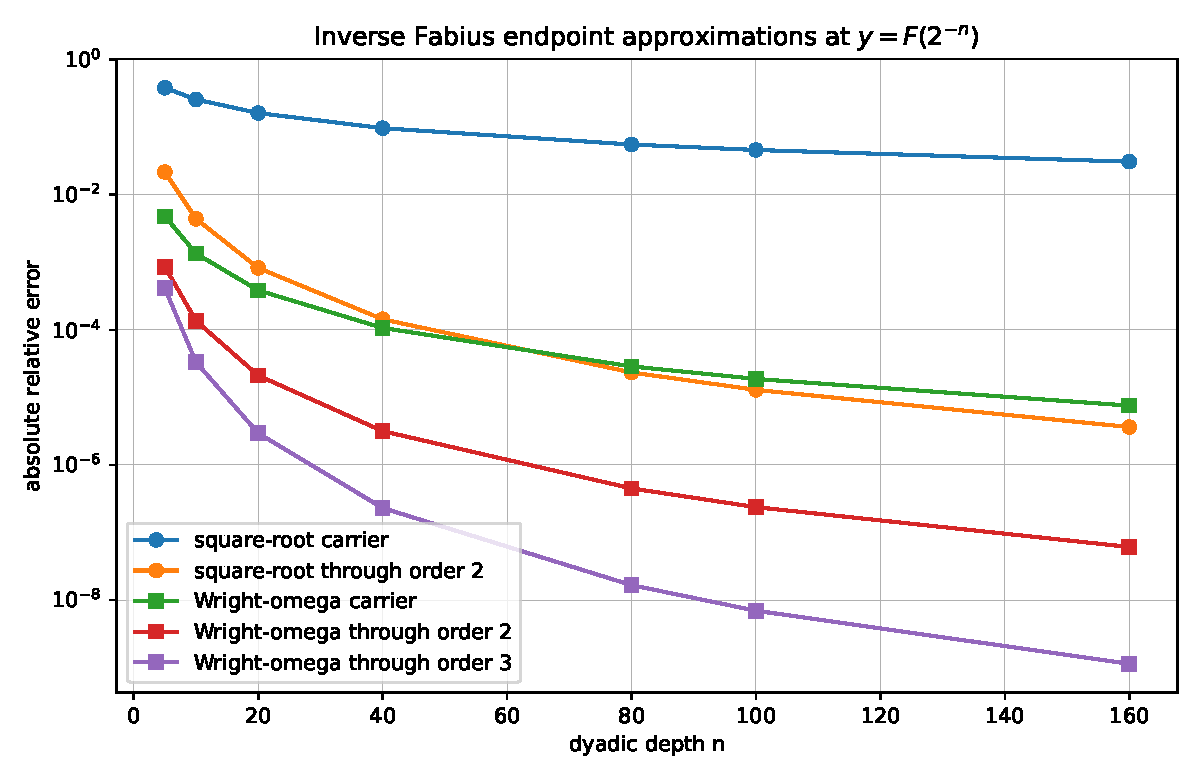
\includegraphics[width=0.78\textwidth]{assets/endpoint/wright-omega/figures/carrier_comparison.pdf}\\[0.3em]
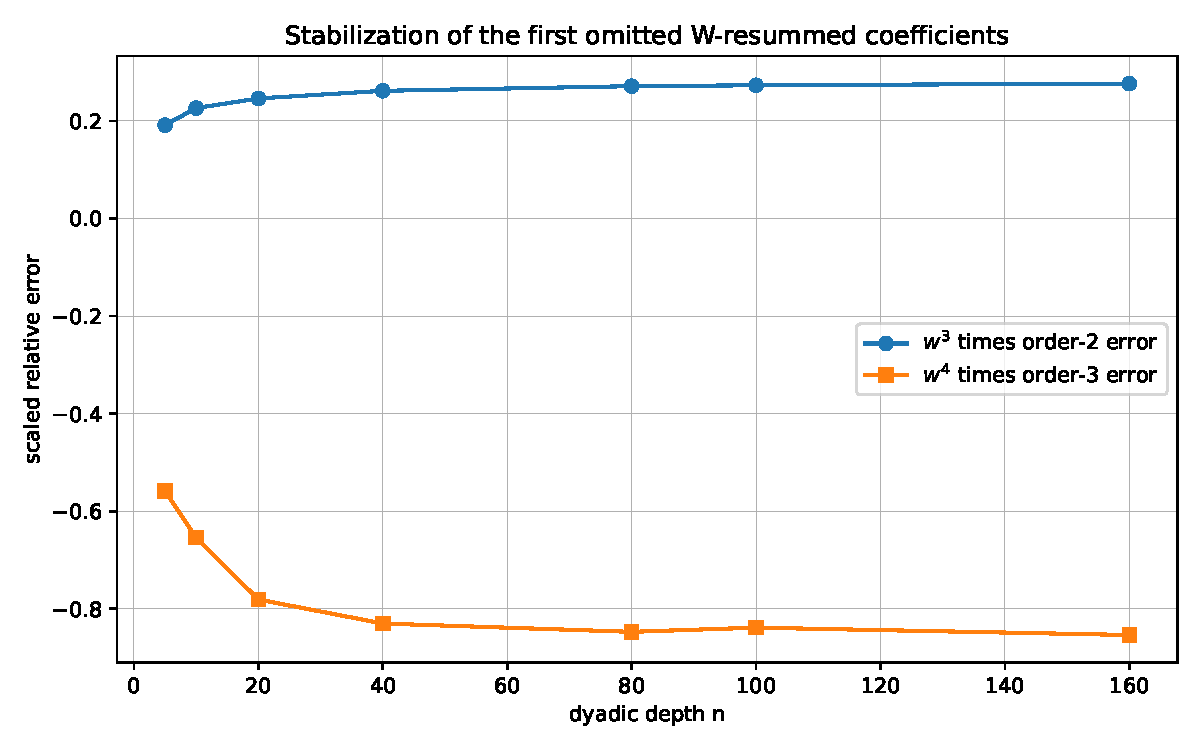
\includegraphics[width=0.78\textwidth]{assets/endpoint/wright-omega/figures/scaled_residuals.pdf}
\caption{Top: absolute relative errors of the $\rho$- and W-carrier
approximants on the exact dyadic quantiles.  Bottom: scaled residuals
after the second and third W-corrections, consistent with the
predicted next powers $w^{-3}$, $w^{-4}$.}
\label{ao:fig:W-figures}
\end{figure}

\begin{remark}[Pre-asymptotic hierarchy]
Since $\Norm{\Psi}_\infty\approx2.13\times10^{-6}$ while
$(h_2^W)^{(0)}=5/24$, the nominally first correction
$h_1^W/w=-\Psi/w$ is numerically \emph{invisible} against
$h_2^W/w^{2}$ until
$w\gtrsim(5/24)/\Norm{\Psi}_\infty\approx10^{5}$, i.e.\
$T\sim3\times10^{9}$.  Practical approximations must therefore
include $h_2^W$ whenever they include $h_1^W$
(cf.\ the table's near-identical first two columns).  This does not
violate asymptotic ordering; one coefficient simply happens to be
extraordinarily small --- the same smallness that makes the phase
oscillation resolvable only at high precision.
\end{remark}

\begin{remark}[Candidate beyond-all-orders scales; heuristic only]
The exact dyadic tail suggests an inverse perturbation on the scale
$w^{-1}e^{-2^{q_\star}}$, where $q_\star$ is the exact saddle coordinate;
replacing it by $\vartheta$ is not uniform, as explained after
\eqref{ao:eq:touchard-jets}.  A second candidate comes from the isolated
linear top-jet contribution \eqref{ao:eq:amplitude-law}.  Combining its
$k$th Fourier factor with
$|\Psihat(k)|$ and optimizing in $k$ places the largest term of that
\emph{single contribution} near
$k_*\sim2(m-1)L/\pi^2$ and suggests the factorial scale
$m!(8/\pi^2)^m$, least term near $m\sim\pi^2w/8$, and exponential size
$e^{-\pi^2w/8}$.

None of these optimizations controls the remaining saddle diagrams.  They may
reinforce or cancel the isolated Fourier mode, and no analytic continuation
of the Borel transform is proved here.  In particular this calculation does
\emph{not} establish an exact limsup, Borel summability, a Borel singularity
at $\pi^2/8$, or a Stokes multiplier.  It records only the candidate constants
used to formulate \cref{ao:conj:gevrey,ao:conj:optimal-truncation,ao:conj:transseries}.
Locating the nearest complex singularity of the bare implicit germ
\eqref{ao:eq:bare-series} is a separate elimination problem and would measure
the carrier's geometric, rather than factorial, coefficient growth.
\end{remark}

\section{The forward saddle engine: constrained partition sums}
\label{ao:sec:saddle}

The inverse formulas consume the periodic forward coefficients
$A_j$.  This chapter closes their construction with a finite
partition formula for the universal Gaussian layer of the saddle
analysis of the Bromwich integral.

Let $s>0$ solve the saddle equation $x=-K'(s)$ and normalize the
saddle jets and their ratios
\begin{equation}
 \varkappa_r=s^{r}K^{(r)}(s),
 \qquad
 \varrho_r=\frac{\varkappa_r}{\varkappa_2}
 \quad(r\ge3).
 \label{ao:eq:saddle-jets}
\end{equation}
Scaling the contour by $t=s(1+\ImaginaryUnit Z/\sqrt{\varkappa_2})$,
$Z\sim N(0,1)$, produces the formal correction factor
\begin{equation}
 \mathcal S=\Expectation\left[
 \Bigl(1+\frac{\ImaginaryUnit Z}{\sqrt{\varkappa_2}}\Bigr)^{-1}
 \exp\Bigl(\sum_{r\ge3}\frac{\varrho_r}{r!}
 \frac{(\ImaginaryUnit Z)^{r}}{\varkappa_2^{(r-2)/2}}\Bigr)
 \right]
 \sim1+\sum_{n\ge1}\frac{C_n}{\varkappa_2^{\,n}},
 \label{ao:eq:S-def}
\end{equation}
the reciprocal factor being the CDF's Bromwich $1/t$ --- deleting it
would produce the \emph{density} coefficients instead.

\begin{theorem}[Constrained-partition formula]
\label{ao:thm:Cn}
For $n\ge1$,
\begin{equation}
 \boxed{\;
 C_n=\sum_{\substack{m_0,m_3,m_4,\dots\ge0\\
 m_0+\sum_{r\ge3}(r-2)m_r=2n}}
 (-1)^{m_0+N/2}\,(N-1)!!\,
 \prod_{r\ge3}\frac{\varrho_r^{\,m_r}}{m_r!\,(r!)^{m_r}},
 \qquad
 N:=m_0+\sum_{r\ge3}rm_r,
 \;}
 \label{ao:eq:Cn-partition}
\end{equation}
a finite sum (the constraint forces $N$ even and $r\le2n+2$).  When
all $\varrho_r$ vanish it reduces to the Gaussian Mills-ratio
coefficients $C_n=(-1)^{n}(2n-1)!!$ --- a sensitive sign and
normalization check, verified symbolically ($-1,3,-15$).  The
logarithmic coefficients
$\log\mathcal S\sim\sum\Lambda_n\varkappa_2^{-n}$ follow
nonrecursively from
\begin{equation}
 \Lambda_n=\sum_{k=1}^{n}\frac{(-1)^{k-1}}k
 \sum_{n_1+\dots+n_k=n,\;n_j\ge1}
 C_{n_1}\cdots C_{n_k},
 \qquad
 \Lambda_1=C_1,\quad
 \Lambda_2=C_2-\tfrac12C_1^{2}.
 \label{ao:eq:Lambda}
\end{equation}
\end{theorem}

\begin{proof}
Expand the reciprocal geometrically ($m_0$ factors of
$-\ImaginaryUnit Z/\sqrt{\varkappa_2}$) and the exponential by multiplicities
$m_r$.  The total inverse half-power of $\varkappa_2$ is
$\tfrac12(m_0+\sum(r-2)m_r)$, giving the constraint; the Gaussian
degree is $N$ with $N-2n=2\sum m_r$ even, so
$\Expectation Z^{N}=(N-1)!!$; the powers of $\ImaginaryUnit$ and the reciprocal's sign
give $(-1)^{m_0+N/2}$; and the exponential series supplies the
multiplicity factorials.  The $\Lambda$ formula is
$\log(1+\cdot)$ composed with the $C$-series.
\end{proof}

The first coefficients are
$C_1=-1-\tfrac12\varrho_3+\tfrac18\varrho_4
-\tfrac5{24}\varrho_3^{2}$ and
\begin{equation}
 C_2=3+\tfrac52\varrho_3-\tfrac58\varrho_4+\tfrac18\varrho_5
 -\tfrac1{48}\varrho_6
 +\tfrac{35}{24}\varrho_3^{2}-\tfrac{35}{48}\varrho_3\varrho_4
 +\tfrac7{48}\varrho_3\varrho_5+\tfrac{35}{384}\varrho_4^{2}
 +\tfrac{35}{48}\varrho_3^{3}
 -\tfrac{35}{64}\varrho_3^{2}\varrho_4
 +\tfrac{385}{1152}\varrho_3^{4}.
 \label{ao:eq:C2}
\end{equation}
With $q=\log_2s$ and $J(q)=K(2^{q})$, the normalized jets are
generated exactly by the operator identity
$\varkappa_r(q)=L^{-r}\prod_{j=0}^{r-1}(D_q-jL)\,J(q)$; inserting
the exact decomposition of $K$ from
\cref{ao:sec:dyadic-completion} and converting from the saddle
coordinate $q$ to the exact Lambert phase completes the pipeline
\begin{equation}
 \Psi
 \;\longrightarrow\;\{\varkappa_r\}
 \;\xrightarrow{\eqref{ao:eq:Cn-partition}}\;\{C_n\}
 \;\xrightarrow{\eqref{ao:eq:Lambda}}\;\{\Lambda_n\}
 \;\longrightarrow\;\{A_j\}
 \;\xrightarrow{\eqref{ao:eq:diagonal-dn}}\;\{d_n\}
 \;\xrightarrow{\eqref{ao:eq:gn-direct}}\;\{g_n\},
 \label{ao:eq:pipeline}
\end{equation}
every arrow a finite differential-polynomial or
coefficient-extraction operation at fixed order.  The raw term count
of \eqref{ao:eq:Cn-partition} grows like an integer-partition function
--- subexponentially --- rather than like all set partitions, which
removes the practical bottleneck to generating $A_3,A_4,\dots$ in
compact Fourier-differential form.

For implementers, the corpus also supplies a second, fully unrolled
closed route to the same $A_j$ (recorded in the third absorbed
source from the archived small-argument study): with the signed
Stirling coefficients $\prod_{r=1}^{n}(z-r)=\sum_mc(n,m)z^{m}$ and
harmonic numbers $\Hnum_n$, the bounded saddle jets are
\begin{equation}
 q_n(u)=(-1)^{n}n!\Bigl(\frac{\Hnum_n}{L}-\frac12\Bigr)
 +\sum_{m=0}^{n}c(n,m)\,\frac{\Psi^{(m+1)}(u)}{L^{m+1}},
 \label{ao:eq:qn-jets}
\end{equation}
the normalized mass coefficients $a_j$ are finite sums over
compositions of $2j$ and subsets weighted by double factorials
$(2j+2\AbsoluteValue S-1)!!$, and
$A_j=\sum_{r\le j}\frac{(-1)^{r-1}}r
\sum_{\mathcal C(j,r)}a_{s_1}\cdots a_{s_r}$ --- an explicit finite
differential polynomial in $\Psi',\dots,\Psi^{(2j)}$ whose top jet
reproduces \eqref{ao:eq:A1-and-topjet}.  The partition engine
\eqref{ao:eq:Cn-partition} and this composition route validate each
other symbolically.

\section{The exact \texorpdfstring{$2$}{2}-adic completion of the
Laplace exponent}
\label{ao:sec:dyadic-completion}

Everything so far is asymptotic in $\rho$.  This chapter is
\emph{exact}: it completes the quadratic--periodic normal form of
$K$ by an explicitly $2$-adic, everywhere-convergent tail, and shows
that the periodic phase and the beyond-all-orders sectors are two
faces of one Mellin kernel.

\subsection{The decomposition and the dyadic Bose tail}

The product \eqref{ao:eq:K-def} gives the dyadic difference equation
$K(2t)-K(t)=\log(1-\EulerE^{-t})-\log t$.  Define the \emph{dyadic Bose
tail}
\begin{equation}
 B(t)=-\sum_{k\ge0}\log\bigl(1-\EulerE^{-2^{k}t}\bigr),
 \qquad
 B(t)=-\log(1-\EulerE^{-t})+B(2t).
 \label{ao:eq:B-def}
\end{equation}

\begin{theorem}[Exact quadratic--periodic--dyadic decomposition]
\label{ao:thm:K-decomposition}
For every $t>0$,
\begin{equation}
 \boxed{\;
 K(t)=-\frac{\log^{2}t}{2L}+\frac12\log t-\CB
 +\Psi(\log_2t)+B(t).
 \;}
 \label{ao:eq:K-decomposition}
\end{equation}
\end{theorem}

\begin{proof}
With $Q(q)=-\tfrac L2q^{2}+\tfrac L2q$ one checks
$Q(q+1)-Q(q)=-Lq$, so
$\Omega(q):=K(2^{q})-Q(q)-B(2^{q})$ is $1$-periodic by the two
difference equations.  The small-$t$ Mellin expansion of $B$
(\cref{ao:thm:mellin-bridge} below) is
$B(t)=\log^{2}(1/t)/(2L)+\tfrac12\log(1/t)+\CB-\Psi(\log_2t)+
\LittleO(1)$, and $K(t)\to0$ as $t\downarrow0$; letting
$q=m+u\to-\infty$ at fixed $u$ identifies
$\Omega(u)=\Psi(u)-\CB$, and periodicity upgrades the identity to
all $q$.
\end{proof}

\begin{theorem}[Exact $2$-adic coefficients]
\label{ao:thm:B-2adic}
For every $t>0$,
\begin{equation}
 \boxed{\;
 B(t)=\sum_{n\ge1}b_n\,\EulerE^{-nt},
 \qquad
 b_n=\frac{2^{\TwoAdicValuation(n)+1}-1}{n},
 \;}
 \qquad
 0<b_n<2,
 \label{ao:eq:B-2adic}
\end{equation}
with the elementary tail enclosure
$0<B(t)-\sum_{n\le N}b_n\EulerE^{-nt}\le2\EulerE^{-(N+1)t}/(1-\EulerE^{-t})$.
\end{theorem}

\begin{proof}
Expand each Bose logarithm and regroup
$B(t)=\sum_{k\ge0}\sum_{m\ge1}m^{-1}\EulerE^{-m2^{k}t}$: the
representations $n=m2^{k}$ are indexed by $0\le k\le\TwoAdicValuation(n)$, with
total weight
$\tfrac1n\sum_{k\le\TwoAdicValuation(n)}2^{k}=(2^{\TwoAdicValuation(n)+1}-1)/n$.
\end{proof}

The first terms,
$B(t)=\EulerE^{-t}+\tfrac32\EulerE^{-2t}+\tfrac13\EulerE^{-3t}
+\tfrac74\EulerE^{-4t}+\tfrac15\EulerE^{-5t}+\tfrac12\EulerE^{-6t}+\cdots$, spike at
powers of two: the exact arithmetic trace of the dyadic scale
hierarchy.  The integer weight $f(n)=nb_n=2^{\TwoAdicValuation(n)+1}-1$
satisfies $f(2n)=2f(n)+1$, $f(2n+1)=1$, and its generating function
obeys the Mahler equation $C(z)=2C(z^{2})+z/(1-z)$, placing the
sectors in the same digital universe as the Thue--Morse and ruler
sequences --- but with geometric accumulation over the full
$2$-adic valuation in place of digit-sum parity.  Note the
crosswalk: $\TwoAdicValuation(n)+1$ is precisely the integer zero order of
$\FourierTwoPi{\RvachevUp}$ that drives the exactness theorems of the companion
volume \emph{Dyadic-Comb Frontiers}; here the same statistic returns
as the arithmetic seed of the beyond-all-orders sectors.

\subsection{One Mellin kernel, two asymptotic ends}

\begin{theorem}[Mellin bridge]
\label{ao:thm:mellin-bridge}
For $\Re s>0$,
\begin{equation}
 \sum_{n\ge1}\frac{b_n}{n^{s}}
 =\frac{\zeta(s+1)}{1-2^{-s}},
 \qquad
 \int_0^\infty B(t)\,t^{s-1}\Differential t
 =\Gamma(s)\,\frac{\zeta(s+1)}{1-2^{-s}},
 \label{ao:eq:mellin}
\end{equation}
and contour shifting in the Mellin inversion gives, for every fixed integer
$M\ge1$, with $R=\log(1/t)$,
\begin{equation}
 B(t)=\frac{R^{2}}{2L}+\frac R2+\CB-\Psi(\log_2t)
 +\sum_{m=1}^{M-1}\frac{(-1)^{m}\zeta(1-m)}{m!\,(1-2^{m})}\,t^{m}
 +\BigO_M(t^{M})
 \qquad(t\downarrow0).
 \label{ao:eq:B-small-t}
\end{equation}
\end{theorem}

\begin{proof}
For $\Re s>0$, Tonelli's theorem applied to absolute values gives
\[
 \sum_{n\ge1}\frac{b_n}{n^s}
 =\sum_{k\ge0}\sum_{m\ge1}\frac{1}{m(m2^k)^s}
 =\zeta(s+1)\sum_{k\ge0}2^{-ks}
 =\frac{\zeta(s+1)}{1-2^{-s}}.
\]
The exact series \eqref{ao:eq:B-2adic} is locally uniformly convergent for
$t>0$.  A second application of Tonelli, followed by
$\int_0^\infty e^{-nt}t^{s-1}\,dt=n^{-s}\Gamma(s)$, proves the Mellin
transform identity.  To make the endpoint bounds explicit, put
$J=\Ceiling{\log_2(1/t)}$ when $0<t\le1$.  For $k\le J$,
$-\log(1-e^{-2^kt})\le C+|\log(2^kt)|$, whose sum is
$O((1+|\log t|)^2)$; for $k>J$, the inequality
$-\log(1-e^{-u})\le C e^{-u}$ for $u\ge1$ and dyadic growth give a bounded
tail.  Thus $B(t)$ has at most quadratic logarithmic growth at zero.  Its
defining series also gives exponential decay at infinity, so Mellin inversion
is valid on every line $\Re s=c>0$:
\[
 B(t)=\frac{1}{2\pi\ImaginaryUnit}
 \int_{c-\ImaginaryUnit\infty}^{c+\ImaginaryUnit\infty}
 \Gamma(s)\frac{\zeta(s+1)}{1-2^{-s}}t^{-s}\,\Differential s.
\]

Shift a rectangular contour to $\Re s=-M-\tfrac12$, choosing its horizontal
edges between the poles on $\Re s=0$.  Stirling's bound gives exponential
decay $e^{-\pi|\Im s|/2}$ for $\Gamma(s)$, whereas $\zeta(s+1)$ has only
polynomial vertical growth.  Thus the horizontal integrals vanish and the
residue series on $\Re s=0$ converges normally.  The pole at $s=0$ has order
three.  The Laurent expansions
\[
 \Gamma(s)=\frac1s-\gamma+
 \left(\frac{\gamma^2}{2}+\frac{\pi^2}{12}\right)s+O(s^2),\qquad
 \zeta(1+s)=\frac1s+\gamma-\gamma_1s+O(s^2),
\]
\[
 \frac1{1-e^{-Ls}}=\frac1{Ls}+\frac12+\frac{Ls}{12}+O(s^3),
 \qquad t^{-s}=e^{Rs}=1+Rs+\frac{R^2s^2}{2}+O(s^3)
\]
show that its residue contribution is
\[
 \frac{R^2}{2L}+\frac R2+\frac L{12}
 +\frac{\pi^2-6\gamma^2-12\gamma_1}{12L}
 =\frac{R^2}{2L}+\frac R2+\CB.
\]
The other zeros of $1-2^{-s}$ are the simple points $s=\chi_k$, $k\ne0$.
Their residues sum, after replacing $k$ by $-k$, to
\[
 \sum_{k\ne0}\frac{\Gamma(-\chi_k)\zeta(1-\chi_k)}{L}t^{\chi_k}
 =-\Psi(\log_2t).
\]
At $s=-m$, $1\le m\le M$, the residue of $\Gamma$ is $(-1)^m/m!$,
so the corresponding term is
\[
 \frac{(-1)^m\zeta(1-m)}{m!(1-2^m)}t^m.
\]
On the new vertical line the denominator is bounded away from zero, and the
same Gamma estimate bounds the remaining integral by $O_M(t^{M+1/2})$.
Retain the residues with $m<M$ and absorb the $m=M$ term and the new-line
integral into $O_M(t^M)$.  This proves \eqref{ao:eq:B-small-t}.
\end{proof}

\begin{statuspanel}{Two faces of one kernel}
The Gamma--zeta phase $\Psi$ (small-$t$ residues at the complex
dimensions $2\pi\ImaginaryUnit k/L$) and the exact $2$-adic exponential sectors
(large-$t$ Dirichlet regrouping) are generated by the \emph{same}
kernel $\Gamma(s)\zeta(s+1)/(1-2^{-s})$.  No new frequencies ever
appear downstream: the entire hierarchy of inverse oscillations
consists of integer convolutions of the modes
$\chi_k$ (\cref{ao:prop:convolutions}), and the beyond-all-orders
remainder is not an opaque error but the explicit arithmetic object
\eqref{ao:eq:B-2adic}.  Comparing the two constant terms independently
recovers the relation $\Csharp+\CB=-\tfrac12\log(2\pi)$ already visible in
\eqref{ao:eq:constants}.
\end{statuspanel}

\subsection{Exact saddle map and ultraflat jets}

\begin{corollary}[Exact $2$-adic saddle map]
\label{ao:cor:saddle-map}
With $t=2^{q}$, the saddle abscissa $x=-K'(t)$ is exactly
\begin{equation}
 \boxed{\;
 x(q)=2^{-q}\Bigl(q-\frac12-\frac{\Psi'(q)}{L}\Bigr)
 +\sum_{n\ge1}\bigl(2^{\TwoAdicValuation(n)+1}-1\bigr)\,\EulerE^{-n2^{q}},
 \;}
 \label{ao:eq:saddle-map}
\end{equation}
the first term the complete algebraic--periodic saddle map, the
second an exact convergent ultraflat correction.  Derivative
bookkeeping is closed: with Stirling numbers of the second kind,
\begin{equation}
 \frac{\Differential^{r}}{\Differential q^{r}}B(2^{q})
 =L^{r}\sum_{n\ge1}b_n
 \sum_{j=0}^{r}
 \genfrac\{\}{0pt}{}{r}{j}\,(-n2^{q})^{j}\,\EulerE^{-n2^{q}},
 \qquad
 t^{r}B^{(r)}(t)=(-1)^{r}\sum_{n\ge1}b_n\,(nt)^{r}\EulerE^{-nt}.
 \label{ao:eq:touchard-jets}
\end{equation}
\end{corollary}

\begin{proof}
Differentiate the exact decomposition \eqref{ao:eq:K-decomposition}.  Since
$q=\log_2t=(\log t)/L$,
\[
 -K'(t)=\frac1t\left(q-\frac12-\frac{\Psi'(q)}L\right)-B'(t).
\]
The series in \eqref{ao:eq:B-2adic} and all of its termwise derivatives
converge uniformly on each half-line $t\ge t_0>0$, so
\[
 -B'(t)=\sum_{n\ge1}n b_ne^{-nt}
 =\sum_{n\ge1}(2^{\TwoAdicValuation(n)+1}-1)e^{-nt}.
\]
Putting $t=2^q$ gives \eqref{ao:eq:saddle-map}.

Ordinary termwise differentiation gives
\[
 t^rB^{(r)}(t)=(-1)^r\sum_{n\ge1}b_n(nt)^re^{-nt}.
\]
For derivatives in $q$, use
$\Differential/\Differential q=L,t\Differential/\Differential t$ and the
operator identity
\[
 (t\Differential_t)^r
 =\sum_{j=0}^r\genfrac\{\}{0pt}{}{r}{j}t^j\Differential_t^j.
\]
Applying it termwise to $e^{-nt}$ proves the first formula in
\eqref{ao:eq:touchard-jets}.  Uniform convergence on compact $q$-intervals
justifies all differentiations and interchanges.
\end{proof}

The jet formulas expose the technical obstacle to naive
hyperasymptotics: each $q$-derivative of an
$\EulerE^{-n2^{q}}$ sector produces powers of $2^{q}$, so the ordinary
inverse-power saddle hierarchy is \emph{not uniform} inside a fixed
dyadic sector; and although the algebraic inversion gives the saddle
coordinate $q_\star(y)=\theta+\BigO(\ell/\rho)$, the induced change
in the exponent $n2^{q_\star}$ is of order
$2^{\theta}\ell/\rho\to\infty$ --- the exact saddle coordinate is
part of the beyond-all-orders datum
(\cref{ao:conj:transseries}).

% Source fragment: All-orders endpoint asymptotics; prefix ao.
\section{Verification}
\label{ao:sec:verification-inv}

The two absorbed packages verify overlapping claims by independent
implementations; both suites live under \nolinkurl{assets/}.

\emph{Symbolic.}  Over algebraically independent symbols
$L,\beta,\Csharp,\ell,P_0,\dots,P_4,A_1,A_1',A_2$, both codes confirm
$d^{\mathrm{diagonal}}_j-d^{\mathrm{triangular}}_j\equiv0$
($j\le3$), the third correction \eqref{ao:eq:d3}, the universal top-log
\eqref{ao:eq:universal-top-log}, and the top-jet transfer
\eqref{ao:eq:inverse-topjet}; the saddle generator reproduces
$C_n=(-1)^{n}(2n-1)!!$ at vanishing $\varrho$ and archives
$C_1,C_2,C_3,\Lambda_2$ (\nolinkurl{generated_coefficients.tex}).

\emph{Exact identities.}  At $70$--$100$ digits, the decomposition
\eqref{ao:eq:K-decomposition} agrees with the defining product for
$K$ to $\sim10^{-16}$ at $t\in\{0.1,1,3,10\}$ (twelve Fourier
modes); the $2$-adic series \eqref{ao:eq:B-2adic} agrees with the
product to $7.5\times10^{-39}$ at $t=0.7$ and
$3.8\times10^{-55}$ at $t=1.5$; the small-$t$ expansion
\eqref{ao:eq:B-small-t} to $\sim4\times10^{-16}$ on
$0.02\le t\le0.2$; and the Dirichlet identity
\eqref{ao:eq:mellin} to the expected algebraic truncation tail with
$5\times10^{4}$ unaccelerated terms.

\emph{Wright-omega layer.}  The third source's suite independently
reconstructs the W-scale $d_m^W,h_m^W,g_m^W$ symbolically from the residual
equation (SymPy; the identities of
\cref{ao:sec:wcarrier} including the $5/24$ cancellation and the
zero-periodic values \eqref{ao:eq:zero-periodic}), verifies the carrier
equation and Newton evaluation of $\omega$, and generates the
carrier-comparison tables of \cref{ao:tab:W-errors} on the same exact
dyadic quantiles at $100$ digits with nine Fourier modes.

\emph{Exact dyadic quantiles.}  With $a_0=1$ and
$a_n=(2^{n}-1)^{-1}\sum_{k<n}a_k/(n-k+1)!$, the repository's exact
values give $y_n=F(2^{-n})=2^{-n(n-1)/2}a_n$ with
$G(y_n)=2^{-n}$ \emph{exactly} --- no inversion error, only the
asymptotic formula is evaluated (at $100$ digits, twelve modes).
Signed relative errors of $G^{[r]}
=\Gzero\exp(\sum_{j\le r}h_j\rho^{-j})$:

\begin{center}
\small
\begin{tabular}{@{}rrrrrr@{}}
\toprule
$n$ & $\rho$ & $\Gzero$ only & through $h_1$ & through $h_2$ & through $h_3$ \\
\midrule
5   & 6.44   & $-3.83\times10^{-1}$ & $7.89\times10^{-2}$ & $-2.17\times10^{-2}$ & $6.41\times10^{-3}$ \\
10  & 12.08  & $-2.57\times10^{-1}$ & $2.69\times10^{-2}$ & $-4.40\times10^{-3}$ & $7.19\times10^{-4}$ \\
20  & 22.82  & $-1.62\times10^{-1}$ & $8.76\times10^{-3}$ & $-8.24\times10^{-4}$ & $7.40\times10^{-5}$ \\
40  & 43.65  & $-9.66\times10^{-2}$ & $2.72\times10^{-3}$ & $-1.43\times10^{-4}$ & $6.96\times10^{-6}$ \\
80  & 84.54  & $-5.53\times10^{-2}$ & $8.05\times10^{-4}$ & $-2.34\times10^{-5}$ & $6.05\times10^{-7}$ \\
120 & 125.08 & $-3.94\times10^{-2}$ & $3.88\times10^{-4}$ & $-7.92\times10^{-6}$ & $1.40\times10^{-7}$ \\
160 & 165.47 & $-3.08\times10^{-2}$ & $2.30\times10^{-4}$ & $-3.64\times10^{-6}$ & $4.92\times10^{-8}$ \\
\bottomrule
\end{tabular}
\captionof{table}{Exact-quantile tests: the new third correction
improves the two-correction error by factors $11$--$74$ across the
tested range.}
\label{ao:tab:dyadic-errors}
\end{center}

\begin{figure}[htbp]
\centering
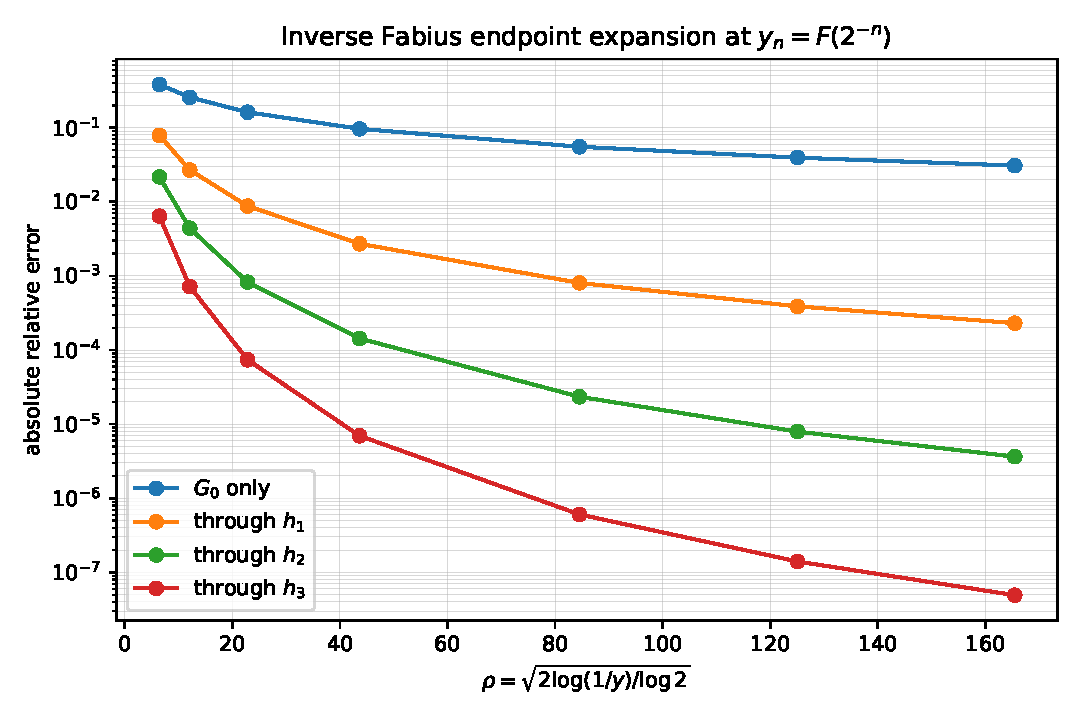
\includegraphics[width=0.78\textwidth]{assets/endpoint/all-orders/figures/endpoint_error_plot.pdf}
\caption{Absolute relative errors on the exact dyadic quantiles;
each added logarithmic correction produces the expected strong
reduction once $\rho$ is moderately large.}
\label{ao:fig:error-plot}
\end{figure}

\begin{figure}[htbp]
\centering
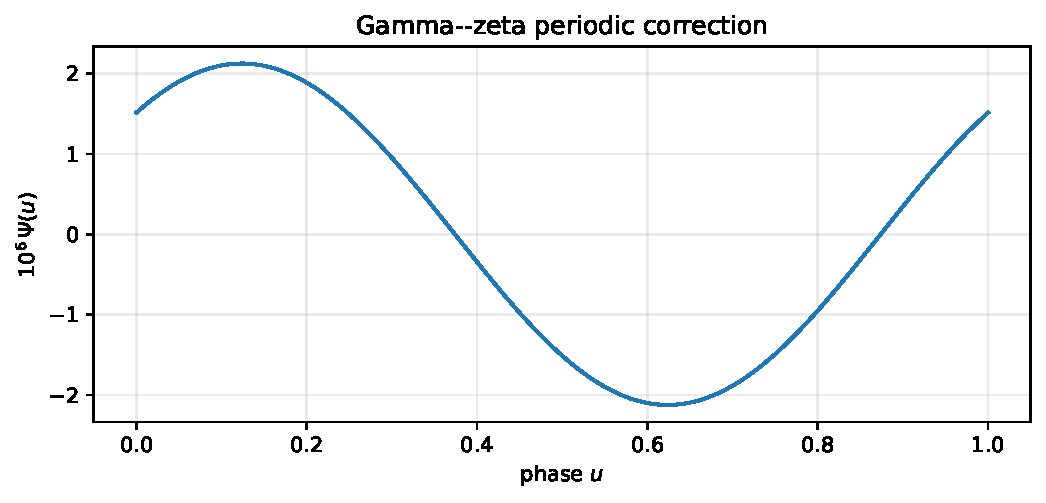
\includegraphics[width=0.72\textwidth]{assets/endpoint/dyadic-completion/figures/psi_periodic.pdf}\\[0.35em]
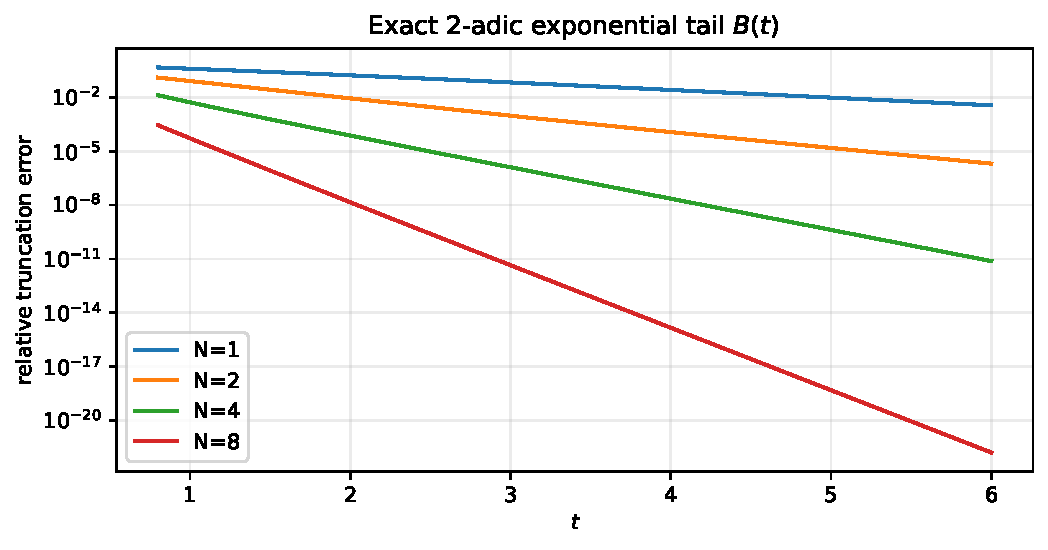
\includegraphics[width=0.72\textwidth]{assets/endpoint/dyadic-completion/figures/dyadic_tail_convergence.pdf}
\caption{Top: the centered Gamma--zeta fluctuation $\Psi$ --- tiny
amplitude, same asymptotic order as the constants.  Bottom: relative
error of $N=1,2,4,8$ terms of the exact $2$-adic series for
$B(t)$, with the elementary enclosure of
\cref{ao:thm:B-2adic}.}
\label{ao:fig:psi-and-tail}
\end{figure}

% Source fragment: All-orders endpoint asymptotics; prefix ao.
\section{Proof details}
\label{ao:app:proof-details}

\emph{Finiteness bookkeeping.}  In \eqref{ao:eq:diagonal-dn} the index-$k$
summand requests $z^{\,n-k}w^{\,k-1}$: no $\Phi$-power beyond
$z^{\,n-k}$, no Taylor jet beyond order $k-1$, and $A_j$ only for
$j\le n-k$; hence $A_{n-1}$ occurs only at $k=1$ --- the key to the
top-jet proof.

\emph{Formal-to-asymptotic transfer.}  Separate the explicit truncated
residual from the value-only error:
\[
 \mathscr F_N(w)=\frac Lz w+\mathcal R_N(w),
 \qquad \mathscr F_N(D)=-E_N(D),
 \qquad |E_N(D)|=O_N(z^N).
\]
Formal cancellation gives
$\mathscr F_N(D^{[N]})=O_N((1+\ell)^Nz^N)$, while
$\inf|\partial_w\mathscr F_N|\ge L/(2z)$ throughout the relevant
$O(\ell z)$ neighborhood.  Applying the mean-value theorem to
$\mathscr F_N$ alone gives
\[
 |D-D^{[N]}|
 \le\frac{2z}{L}
 \bigl(|E_N(D)|+|\mathscr F_N(D^{[N]})|\bigr)
 =O_N((1+\ell)^Nz^{N+1}).
\]
No derivative of $E_N$ is assumed.  This is the gain-of-one-power argument
that lets a forward expansion through $A_{N-1}$ certify an inverse
expansion through $d_N$.  The map
$\lambda\mapsto\lambda\EulerE^{-L\lambda}$ then transfers phase error to
relative inverse error of the same order.

% Source fragment: All-orders endpoint asymptotics; prefix ao.
\section{Conjectures and frontier directions}
\label{ao:sec:conjectures-inv}

\begin{conjecture}[Gevrey-one growth]
\label{ao:conj:gevrey}
For every $0<\sigma'<\pi/(2L)$ there are $C,A>0$ such that
\[
 \|d_n^W\|_{\sigma'}+\|h_n^W\|_{\sigma'}+
 \|g_n^W\|_{\sigma'}\le CA^nn!\qquad(n\ge1).
\]
Writing a $\rho$-coefficient as
$p_n(\ell,\theta)=\sum_rp_{n,r}(\theta)\ell^r$, the same estimate holds
for the coefficient norm $\max_r\|p_{n,r}\|_{\sigma'}$, for each of
$p_n=d_n,h_n,g_n$.  The calculation in the preceding heuristic suggests
$8/\pi^2$ as a candidate exponential constant for one linear contribution,
but this conjecture asserts only Gevrey order one, not that constant and not
Borel summability.
\end{conjecture}

\begin{conjecture}[Optimal truncation]
\label{ao:conj:optimal-truncation}
Fix $u\in\RealNumbers/\IntegerNumbers$ and approach the endpoint along a
W-phase-locked sequence $\vartheta\equiv u\pmod1$.  If the leading
saddle-resurgent multiplier at that phase is nonzero, then the least term of
the W-series occurs at
$N_{\mathrm{opt}}=(\pi^2/8+o(1))w$, and truncation there has relative
remainder $R_u(w)$ satisfying
\[
 \log|R_u(w)|=-\left(\frac{\pi^2}{8}+o(1)\right)w.
\]
The qualification on the multiplier allows exceptional phases at which the
first sector cancels.  No summability assertion is included.
\end{conjecture}

\begin{conjecture}[Sharp strip inheritance]
\label{ao:conj:strip-sharp}
Every nonconstant periodic coefficient occurring in
$d_n,h_n,g_n,d_n^W,h_n^W,g_n^W$ has maximal open strip
$|\Im\theta|<\pi/(2L)$, the maximal strip of $\Psi$, unless its boundary
singularities cancel by an algebraic identity.  In particular the generic
coefficient at each inverse order has Fourier exponential type exactly
$\pi^2/L$ rather than merely at least that type as proved in
\cref{ao:prop:strip}.
\end{conjecture}

\begin{conjecture}[Nonconstant phase at every order]
\label{ao:conj:nonconstant-phase}
For every $n\ge1$, at least one nonzero Fourier coefficient of each
$d_n(\ell,\cdot),h_n(\ell,\cdot),g_n(\ell,\cdot)$ is a nonzero polynomial in
$\ell$; equivalently, none of the three coefficients is phase-blind for all
$\ell$.  Likewise each of $d_n^W,h_n^W,g_n^W$ is nonconstant in its phase.
The formal top-jet law proves that these differential polynomials are not
formally constant; the remaining content is to exclude an identity after
substitution of the particular Gamma--zeta function $\Psi$.
\end{conjecture}

The geometry of the joint phase profiles---immersion, self-intersection, and
possible embeddings after several coefficients are recorded---is a separate
problem and is not part of the preceding nonconstancy conjecture.

\begin{conjecture}[Two-level exponentially improved transseries]
\label{ao:conj:transseries}
After truncating the algebraic W-series at its least term, the relative
remainder decomposes into two asymptotically distinct families.  The first is
a saddle family on scales $e^{-c_jw}$ determined by large-order asymptotics
of the forward coefficients $A_j$.  The second is an ultraflat family on the
exact scales
\[
 \exp(-n2^{q_\star(y)})\qquad(n\ge1),
\]
where $q_\star(y)$ is the exact saddle coordinate of
\eqref{ao:eq:saddle-map}, not the leading phase $\theta$.  At each fixed
ultraflat product order, its arithmetic coefficient sequence belongs to the
finite Dirichlet-convolution algebra generated by
$b_n=(2^{\TwoAdicValuation(n)+1}-1)/n$; equivalently its Dirichlet series is a
finite linear combination of products of shifted copies of
$\zeta(s+1)/(1-2^{-s})$.  The conjecture asserts this scale and coefficient
algebra, but neither Borel summability nor particular Stokes constants.
\end{conjecture}

\begin{conjecture}[Universal diagonal inversion class]
\label{ao:conj:universal-class}
Let $a>0$.  Suppose an endpoint CDF has a strictly monotone exact phase
$\lambda\to\infty$ and a forward expansion
\[
 -a\lambda^2+b\lambda-c\log\lambda+C+P(\lambda)
 +\sum_{j<N}A_j(\lambda)\lambda^{-j}+R_N(\lambda),
\]
where $P,A_j$ are periodic and holomorphic on a common strip, the remainders
and every fixed finite set of their phase derivatives are uniform, and the
phase equation has derivative $2a\lambda+O(1)$ bounded away from zero.  Then
its inverse has a unique diagonal expansion with polynomial logarithms,
phase-locked limits, and Bell conversion; the highest logarithms depend only
on $a$ and $c$.  Any newest-jet conclusion additionally requires a stated
top-jet law for the forward $A_j$.

For the separate base-$b>1$ product of uniform smoothing factors, the exact
digital tail has coefficients
$(b^{\nu_b(n)+1}-1)/((b-1)n)$, Mellin kernel
$\zeta(s+1)/(1-b^{-s})$, and period one in $\log_b$.  The conjectural part is
that the preceding analytic hypotheses and inverse package hold uniformly in
this base-$b$ family; the coefficient regrouping itself is an elementary
finite-valuation calculation.
\end{conjecture}

Concrete projects: generate $A_3,A_4$ compactly through the pipeline
\eqref{ao:eq:pipeline} and make $g_4,g_5$ explicit in $\Psi$ alone;
prove weighted Wiener-algebra bounds uniform in phase; run optimal
truncation experiments to see whether the first visible
beyond-all-orders scale is saddle-resurgent or the far smaller
dyadic one; quantify the uniform-in-$m$ breakdown of the derivative
law \eqref{ao:eq:two-term-derivative}; locate the nearest complex
critical values of $F$ (the analytic continuation radius of $G$ and
the Borel singularities); and build certified few-mode
Fourier-polynomial coefficient tables
$g_n\approx\sum_{r\le n}\sum_{\AbsoluteValue k\le K}c_{n,r,k}\ell^{r}
\EulerE^{2\pi\ImaginaryUnit k\theta}$ that, with one Newton step on the exact
functional equation, give a fast globally certified quantile
algorithm.

\begin{statuspanel}{Lean formalization roadmap}
Four layers, the first three purely formal:
(1) a two-scale coefficient ring (truncated series over
$\RealNumbers[\ell]\otimes C^\infty(\RealNumbers/\IntegerNumbers)$, closure under composition, log,
exp); (2) parameterized Lagrange inversion
$[t^{k}]W=\tfrac1k[w^{k-1}]\Phi^{k}$ and the diagonal specialization
\eqref{ao:eq:diagonal-dn}; (3) the Gaussian contraction
\eqref{ao:eq:Cn-partition} over an algebraic moment functional, and the
$2$-adic regrouping and Dirichlet identities of
\cref{ao:sec:dyadic-completion} (a bijection and two Tonelli
arguments); (4) the analytic transfer
(\cref{ao:app:proof-details}) from formal cancellation to the
fixed-order remainder.  The degree/top-jet filtrations of
\cref{ao:sec:structure} are finite combinatorics on top of (2).
\end{statuspanel}

\appendix
